
\documentclass{article}
\usepackage[utf8]{inputenc}
\usepackage{physics}
\usepackage{enumitem}
\usepackage{listings}
\usepackage[margin=0.5in]{geometry}
\usepackage{graphicx}
\usepackage{float}
\graphicspath{ {Images/} }
\usepackage{amsmath}
\newcommand{\tens}[1]{%
  \mathbin{\mathop{\otimes}\displaylimits_{#1}}%
}
%\usepackage[final]{pdfpages}


%\usepackage[spanish]{babel}    
\usepackage[T1]{fontenc}
\usepackage{natbib}
%\usepackage{array}
%\usepackage{gensymb}
\usepackage{indentfirst}
%\usepackage[table,xcdraw]{xcolor}


% Title page

\title{Atomic Physics Lab}
\author{Joshua Levy\\Lab Partner: Alex Chuang}
\date{February 2017\newpage}


\begin{document}

\maketitle

\section{PreLab and MidLab Sign Offs}
\begin{center}

\includegraphics[scale = 0.28]{JoshATM1.jpg}
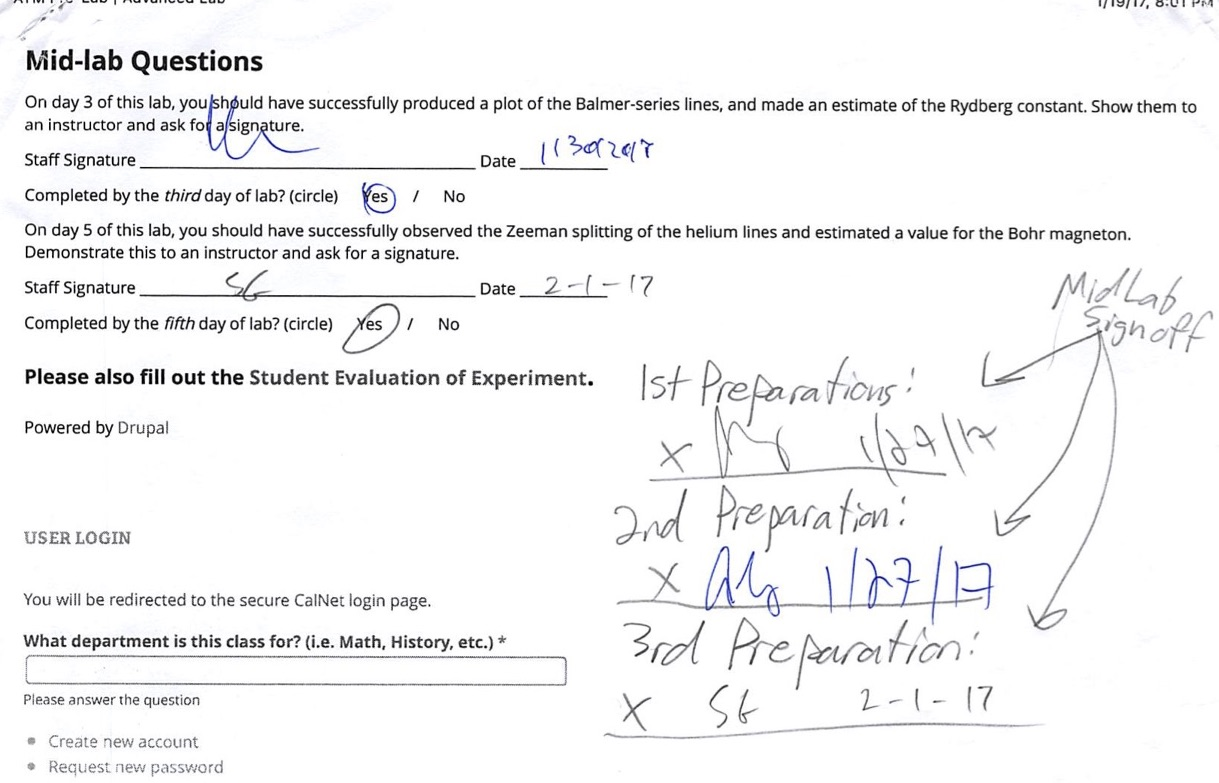
\includegraphics[scale = 0.28]{JoshATM2.jpg}
\end{center}

\newpage


\section{Abstract}
    My partner and I explored the effects of the Balmer Series of hydrogen and observed Zeeman splittings in the red and yellow spectral lines of Helium. We found the wavelengths of the spectral lines of Hydrogen and plotted their wavenumber verses $\frac{1}{n^2}$, where n is the quantum number transitioning down to the n = 2 state. We did this to measure the values of the Rydberg constant, R, which we found to be  and the series limit R/4, which we found to be $1.099*10^{-03} \pm 1.3*10^{-06} \buildrel _\circ \over {\mathrm{A}}^{-1}$ and $2.7*10^{-04} \pm 4.7193*10^{-08} \buildrel _\circ \over {\mathrm{A}}^{-1}$ respectively. For the Zeeman effect, we compared the distances between interference fringes between $\sigma$ components and $\pi$ components, and measured the corresponding magnetic field in order to find the ratio of energy splittings divided by the external magnetic field and the value of the bohr magneton ($\mu_B$), which were found to be $5.06*10^{-5} \pm 1.1*10^{-6} \frac{cm^{-1}}{gauss}$ and $1.00501*10^{-23} \pm 2.11^{-25} \frac{J}{T}$ respectively. In both experiments, the accepted values for R, R/4, and the energy splitting ratio and $\mu_B$ did not agree within the uncertainty bounds of the experimental values, but the relative errors between the observed and expected values were remarkably low.


\section{Introduction}
    In this experiment, we studied the spectral lines in hydrogen and measured the Zeeman effect in a single spectral line of helium.\\
    \subsection{Balmer Series}
        The quantization of light was first uncovered by Planck \cite{purd}, who found that light could only be emitted or absorbed in discrete chunks of energy given by:
        \begin{equation}
            E = hf = \frac{hc}{\lambda}
        \end{equation}
        where E is the energy of the emitted/absorbed photon, f is the frequency of light, c is the speed of light, $\lambda$ is the wavelength and h is the Planck's constant. Einstein showed that this quantization of energy could explain other effects such as the photoelectric effect, where one could shine light on a surface to cause the emission of electrons and other free carriers \cite{purd}. Bohr synthesized these ideas and his knowledge of the atom to find a new theory for the atomic structure of the atom. In classical physics, an electron orbiting an atom would be under constant acceleration and would have to emit radiation. However, Bohr proved this to be untrue, and showed that electrons did not emit radiation as it orbited around the nucleus of an atom. Furthermore, his theory was that the orbits of an electron and the energy of the atomic configuration were both quantized, and that radiation was absorbed by an electron when it jumped to a higher energy level (quantum state) and radiation was emitted when it jumped down to a lower level. This radiation was quantized according to how large the energy jump was, and the frequency or wavelength was determined to be in accordance with the above equation \cite{atm}. The probabilistic theory of quantum mechanics disagreed with some of Bohr's notions, but also found this similar quantization of energy levels. The Balmer series describes energy transitions from higher energy levels to the second energy level in hydrogen. Because these energy levels are quantized, and quantized light is emitted during energy level jumps, we should see that all of the light emitted (a spectrum) has certain frequencies or wavelengths. We chose to observe the Balmer series because the wavelengths in question are mostly in the visible spectrum, and each of these quantized wavelengths correspond to certain colors. These transitions are described by the equation:
        \begin{equation}
            \frac{1}{\lambda} = R*(\frac{1}{2^2} - \frac{1}{n^2})
        \end{equation}
        where R is the Rydberg constant, the 2 represents the quantum number of the second energy level (the level that is being transitioned to), and n represents the energy level (n$>$2) that is being transitioned from. The derivation of this equation will be outlined in the theory section. In our experiment, we will observe the wavelengths of hydrogen (i.e. identify the lines of the Balmer Series), which correspond to transitions from certain energy levels described by n, and we will find a linear relationship between $\frac{1}{\lambda}$ and $\frac{1}{n^2}$. Finding such a relationship will allow us to find the Rydberg constant and the series limit $\frac{R}{4}$ (when n $\rightarrow \infty$), which we can compare to accepted values to confirm the aforementioned theory.\\\indent We will do this by passing  emitted light from a hydrogen lamp through a monochromator, a device that disperses the light into its wavelengths, and then measuring the emitted light's wavelengths by changing the wavelength that we are observing and finding the intensity of the light at all wavelengths (we do this using a procedure that will be described in the procedure section). The wavelengths where the intensity peaks will be our Balmer Series wavelengths.
        
        \subsection{Zeeman Effect}
        The Zeeman Effect is largely founded upon the principles of degenerate perturbation theory. The theory of probabilistic quantum mechanics allows you to find the energy levels of certain quantum states. However, these energy levels can be degenerate, that is, there can be many quantum numbers (eg. n, l j, s) to describe a specific energy level. For instance, states said to be doubly degenerate have two possible quantum states for that particular energy level. Perturbations, that is, small changes in the Hamiltonian describing the energy of the quantum system, can cause these degeneracies to lift, such that there are no longer as many degenerate quantum states for a given energy. Instead, what was once one energy level now splits into many, each with their own quantum states. The Zeeman effect describes one such quantum system. In this effect, the energy levels of a specific atomic configuration are split because the atoms are placed in the presence of a magnetic field. The atoms can be treated as magnetic dipoles, and these dipoles have associated dipole moments that rely on their total angular momentum. The dipoles interact with the magnetic field, and create small perturbations of the atomic energy levels, which in turn lift the degeneracies of these energy levels. Such a perturbation (in the linear realm, small compared to the other energy levels described by the hamiltonian) has been found to be:
        \begin{equation}
            \Delta E = \mu_B g_j m_j B
        \end{equation}
        where $\Delta E$ is the quantized splitting of the energy levels about the once degenerate energy level (i.e. $\Delta E$ is the change of energy from the original degenerate energy line after the magnetic field was introduced), $\mu_B$ is the bohr magneton (a principle unit of magnetic dipole moment), g is the Landé g-factor, $m_j$ is the z-component of the total angular momentum (which is quantized) and B is the magnitude magnetic field (which points in an arbitrary z-direction).\cite{purd}\\\indent
        Now, instead of jumping between the original atomic energy levels, such as that described for the Balmer Series when absorbing and emitting photons, the jumps can occur between  quantized energy level splittings so as long as the jump is on the order of energy transitions of our unperturbed atomic system. The diagram below details such transitions \cite{atm}:
        \begin{figure}[H]
    \centering
    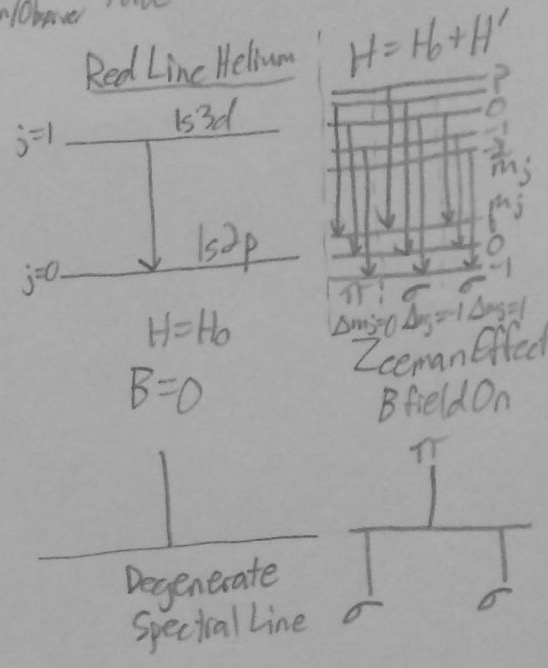
\includegraphics[scale = 0.2]{ATM1d.jpg}
    \caption{}
    \label{fig:my_label}
\end{figure} 
        Therefore, since there is a direct relationship between the wavelength of the emitted light and the energy of an emitted photon (eq.(1)), the spectrum of light we observe also splits. \\\indent The experiment being conducted here will measure the magnitude of these energy splittings in Helium (about the color red, i.e. discover how far red splits apart) once the excited Helium is placed in a magnetic field. The red light splits into three lines, two have slightly higher and lower wavelengths than red respectively and the third line does not change from its original. Light generated from excited Helium atoms in the presence of a magnetic field is sent through various optical instruments, including an instrument that generates circular diffraction patterns, and then sent to a camera, where we can measure the distances between intensity peaks in these circular patterns. We will measure the distance between intensity peaks in the diffracted pattern without the presence of a magnetic field and compare this value to the distance between peaks in the presence of a magnetic field (one peak should split into two to correspond with these energy splits, with the central third one being filtered out). We will use the ratio of these values to help us compute the magnitude of these energy level splits and also measure an experimental value for the bohr magneton (specifics to be described in the theory).

\section{Theory}
    \subsection{Balmer Series}
        % QM derivation
        In Bohr's derivation of the energy levels of an atom, he made the aforementioned assumptions described in the introduction, and then applied the following expressions:
        \begin{equation}
            F_e = \frac{Ze^2}{r^2} = \frac{m_ev^2}{r} = F_c
        \end{equation}
        equating the Coulomb force of an electron orbiting a nucleus (charge Ze) to the centripetal force of the orbit (assumed circular, but later generalized). Note e is the charge of the electron, r is the orbital radius, $m_e$ is the electron's mass, and v is the velocity of the electron.
        \\\indent
        Bohr's theory assumed that the angular momentum of the electron was quantized according to:
        \begin{equation}
            L = m_evr = n\hbar
        \end{equation}
        where $\hbar = \frac{h}{2\pi}$ and n = 1, 2, 3 ...\\\indent Plugging in the value of v found by rearranging eq.(5) into the expression in eq.(4) and solving for r yields:
        \begin{equation}
            r = \frac{n^2\hbar^2}{m_ee^2Z}
        \end{equation}
        The energy of the system in orbit is (T and V are kinetic and potential energy respectively):
        \begin{equation}
            E = T + V = \frac{m_ev^2}{2} + \frac{-Ze^2}{r}
        \end{equation}
        Plugging in the earlier found expressions for r and v, and correcting for reduced mass (elliptical orbits), we see the energy levels and the quantization of light derived from Bohr's theory: 
        \begin{equation}
            E_n = \frac{-2\pi^2\mu e^4 Z^2}{h^2 n^2}
        \end{equation}
        \begin{equation}
            \Delta E = \frac{-2\pi^2\mu e^4 Z^2}{h^2}*(\frac{1}{m^2}-\frac{1}{n^2}) = hf
        \end{equation}
        where $\Delta E$ is the energy of light emitted from the energy transition of the atom, n = 1, 2, 3 ... and m = 1, 2, 3 ... and $\mu$ is the reduced electron mass of the system. Z helps describe the change of the nucleus, and m and n are integers that describe the transition of the electron to a new state based on the emitted/absorbed photon (quantized light particle).\\\indent However, his model was incorrect in his expression of quantized angular momentum ($L\neq n \hbar$). The probabilistic theory of Quantum Mechanics corrected this. It treated a quantum state as a probability amplitude, where the act of measuring this state helps find something out about the system, whether it be the energy of the system, the total or orbital angular momentum, the spin, and so on and so forth. The hamiltonian for our quantum system is:
        \begin{equation}
            H = T + V = \frac{p^2}{2m_e} + \frac{-Ze^2}{r} = -\frac{\hbar^2}{2m_e}\nabla^2 + \frac{-Ze^2}{r}
        \end{equation}
        $m_e$ is the mass of the electron.\\
        If we act this Hamiltonian on the quantum state:
        \begin{equation}
            H \ket{\psi} = (-\frac{\hbar^2}{2m_e}\nabla^2 + \frac{-Ze^2}{r}) \ket{\psi} = E\ket{\psi}
        \end{equation}
        where $\ket{\psi}$ is the three dimensional probability amplitude $\ket{\psi} = \psi(\vec{r})$ and it is a linear superposition of infinitely many eigenstates:
        \begin{equation}
            \ket{\psi} = \sum_{n=1}^\infty c_n \ket{\psi_n}
        \end{equation}
        where each $\ket{\psi_n}$ solves the rearranged linear differential equation: 
        \begin{equation}
            (-\frac{\hbar^2}{2m_e}\nabla^2 + \frac{-Ze^2}{r} - E_n) \ket{\psi_n} = 0
        \end{equation}
        We solve this equation for $\ket{\psi_n}$, and find that the eigenvalue of the equation, $E_n$ is equal to the same expression as in eq.(8) (save for the reduced mass). So eqs.(8-9) are both valid. We can use eq.(9) to find the change in atomic energy associated with a transition/emission/absorption of a photon. If we set Z = 1 and set m = 2, we find the energy of a photon associated with transitions from energy levels of $n = 3, 4, 5, ...$ to m = 2, which describes the Balmer Series. We take this energy and divide by h*c to find the Rydberg formula:
        \begin{equation}
            \frac{1}{\lambda} = R*(\frac{1}{2^2} - \frac{1}{n^2})
        \end{equation}
        where R is the Rydberg constant and equals $\frac{2\pi^2\mu e^4}{h^3c} \approx$ 109,677.581 $cm^{-1}$ for hydrogen. For our experiment, we expect to be able to find R and the series limit $\frac{R}{2^2}$ by taking measurements of the wavelength, plotting $\frac{1}{n^2}$ vs. $\frac{1}{\lambda}$, and fitting a line to the data. We can find R by taking the negative value of the slope of the best fit line and the series limit by finding the y-intercept of the line.  \cite{atm}
      
        
    \subsection{Zeeman Effect}
    The hamiltonian for our quantum system can be described by:
    \begin{equation}
        H = H_o + H'
    \end{equation}
    where $H_o$ is a hamiltonian that returns degenerate eigen energy states that satisfy the potential for a given atom ($H_o = T + V$). This is essentially similar to the Hamiltonian used to derive the energy levels of the hydrogen like atom (which can include electron-electron interactions, spin-orbit coupling and relativistic effects, amongst others). We do not care about this part, as the splittings lay in the perturbed hamiltonian term $H'$ (resulting from a magnetic dipole in the presence of a magnetic field).
    \begin{equation}
        H' = -\vec{\mu} \cdot \vec{B}
    \end{equation}
    where $\vec{B}$ is the magnetic field acting on the magnetic dipole $\vec{\mu}$, which equals:
    \begin{equation}
        \vec{\mu} = \mu_B * g_j * \vec{j}
    \end{equation}
    where $\vec{\mu}$ is related to $\vec{j}$, the total angular momentum of the system. Assuming $\vec{B}$ points in the $\hat{z}$ direction, and eq.(16) can be expressed as:
    \begin{equation}
        H' = -\mu_B g_j \vec{j} \cdot \vec{B} = -\mu_B g_j m_j B = \Delta E
    \end{equation}
    where $m_j$ is the z-component of the total angular momentum (or component pointing along the magnetic field) and can take on integer values between -j and j. Plugging H into our eigenvalue equation with a quantum state described by quantum numbers ($\ket{nljm_j}$, l describes angular momentum) and we get the following result:
    \begin{equation}
        H \ket{nljm_j} = (H_o + H')\ket{nljm_j} = (E_{nl} - \mu_B g_j m_j B)\ket{nljm_j}
    \end{equation}
    where $E_{nl}$ is the degenerate energy level that largely characterizes the atomic energy levels (and main spectra) for particular elements (from Coulomb and fine/hyperfine splittings as well as electron-electron interactions), and $\Delta E = \mu_B g_j m_j B$ is the extra energy perturbation resulting from the magnetic field. $E_{nl}$ can be found on an energy level diagram, while $\Delta E$ is the splitting in question which results in new spectral lines to be formed around the main degenerate line when the spectrum is observed. We see an example of this in the figure below:\\
    \begin{figure}[H]
    \centering
    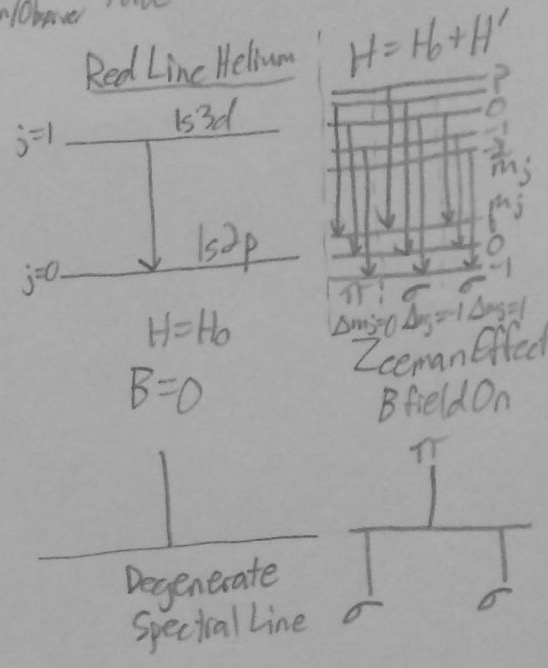
\includegraphics[scale = 0.2]{ATM1d.jpg}
    \caption{}
    \label{fig:my_label}
\end{figure}\\
    In this experiment, we are mostly concerned with analyzing the red line of helium, so its energy level diagram will serve as our example. The figure below is a diagram of the helium atomic energy levels.\\
    \begin{figure}[H]
    \centering
    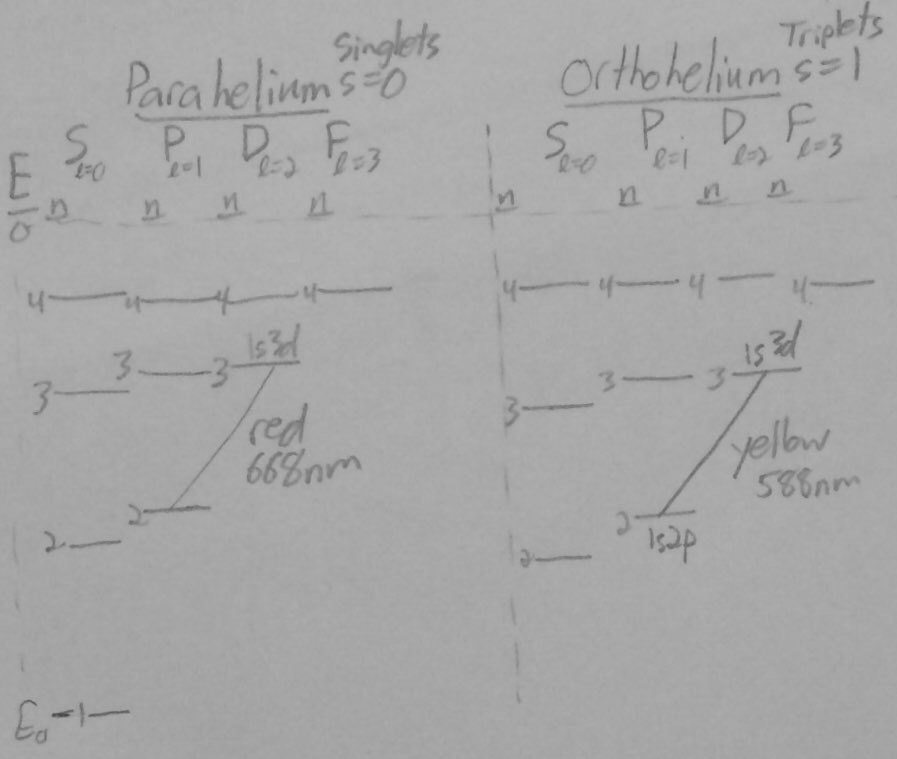
\includegraphics[scale = 0.2]{ATM1c.jpg}
    \caption{}
    \label{fig:my_label}
\end{figure}\\
    As you can see in the figure above, we see that the color red is produced when the optic electron (the electron that is not tightly bound to the nucleus) jumps from the 1s3d state to the 1s2p state (total angular momentum, emitting a photon with frequency equal to $\frac{\Delta E}{h}$. \\ To the right of this energy transition are the energy levels of the Zeeman splittings. For each j-value (total angular momentum), there are 2j+1 possible values of the z-component of angular momentum $m_j$. The perturbed Hamiltonian H’ causes each j-value of energy to split into 2j+1 states, ranging from j, j-1 … -j, by integer values. 
    In this experiment, we generate the light by using a helium lamp. Electrons travel from the cathode to the anode of the lamp, subject to a certain potential,  and their collisions with Helium atoms along the way excite these atoms and cause the optical electrons to jump up from j=1 to j=2. Then the electron spontaneously jumps down back to a lower state (j=2 to j=1) transition and light is emitted. The possible transitions of the electron are limited due to principles involving the conservation of angular momentum involved in the absorption and emission of photons. Such an analysis will not be discussed here, but the following expressions are the selection rules for energy transitions:
    \begin{equation}
        \Delta l = \pm 1; \Delta j = \pm 1, 0; \Delta m_j = \pm 1, 0
    \end{equation}
    We see that the possible $\Delta m_j$ changes correspond to three possible values of our perturbation (above figure). When $\Delta m_j$ = 0, no energy change occurred, and when $\Delta m_j = \pm 1$, the energy of a specific transition is either a little higher or a little lower. Because the energy of a transition corresponds to the wavelength of the emitted light, the wavelength of light will deviate slightly from its original spectral location for these transitions, by the same amount above and below the line. We call the spectral emission line that resulted from a $\Delta m_j$ = 0 transition a $\pi$-component line (which overlaps with the original degenerate line), and one that resulted from a $\Delta m_j = \pm 1$ transition is a $\sigma$-component line. Because the $\sigma$ and $\pi$-components are linearly polarized in different orientations when viewed from an angle perpendicular to the magnetic field's orientation, a polarizer can be used to eliminate either the $\pi$ components (we do this in our experiment) or the $\sigma$ components (we keep these components). Additional visual aids can be seen in the above and below figures. \begin{figure}[H]
    \centering
    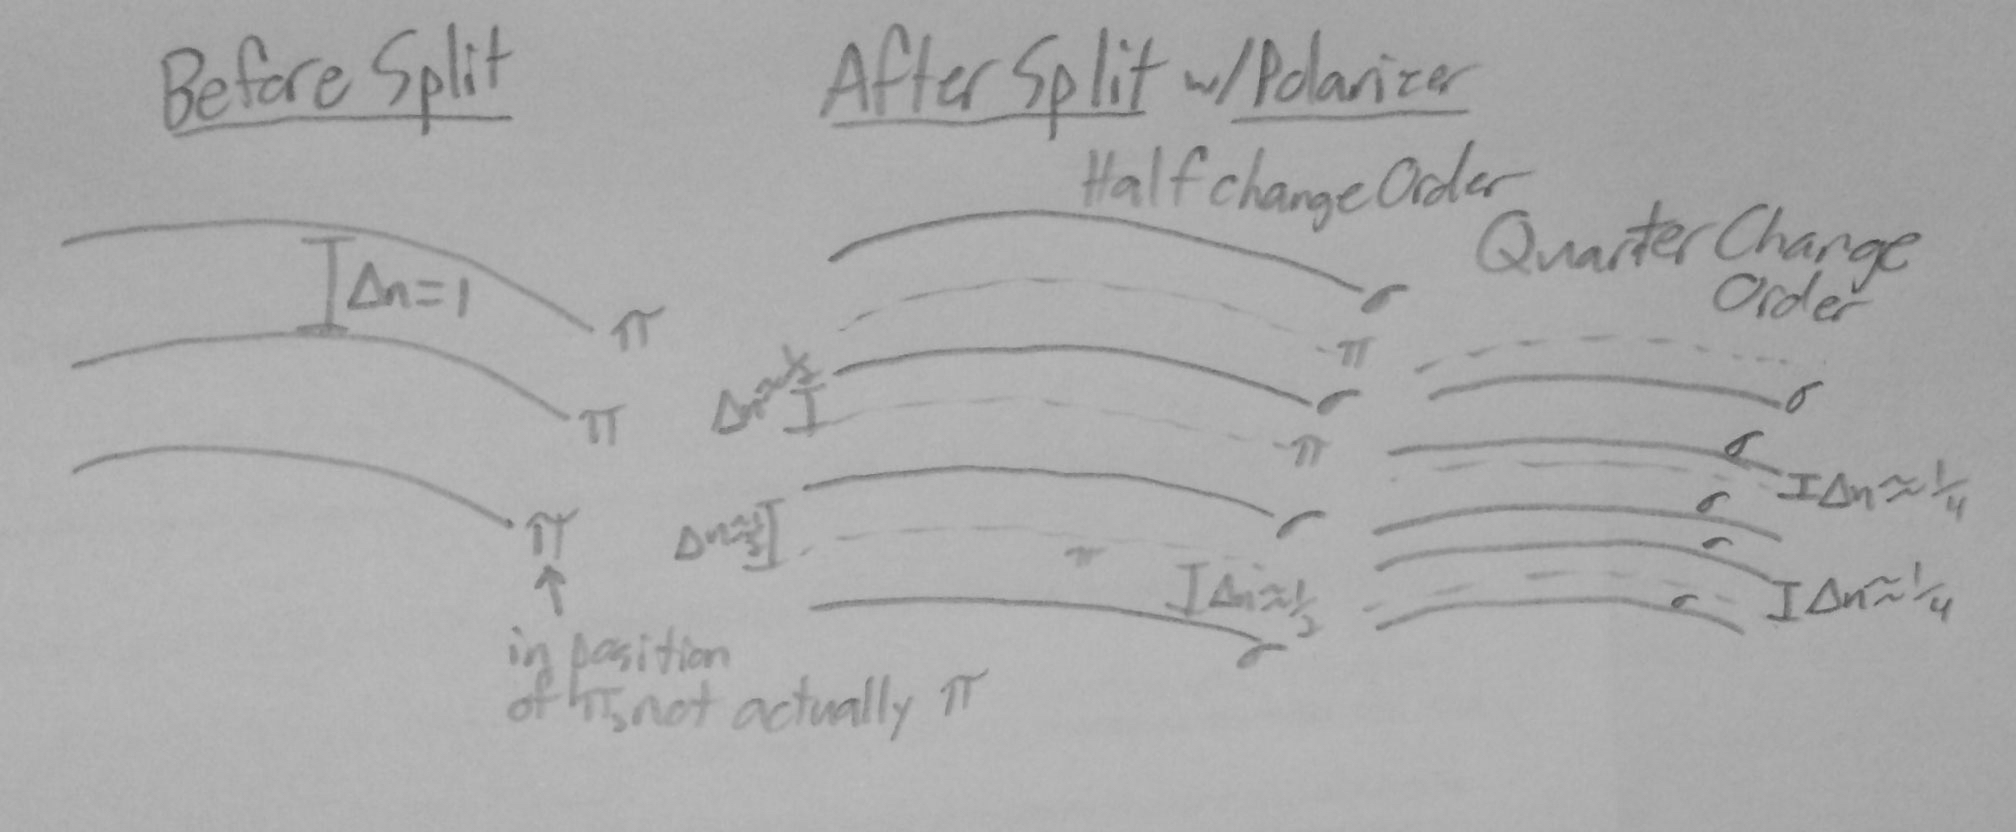
\includegraphics[scale = 0.2]{ATMn.jpg}
    \caption{}
    \label{fig:my_label}
\end{figure}
    An increment of energy for the Zeeman splitting is given by $\Delta \sigma = \frac{\Delta E}{hc} = \frac{\mu_B g_j \Delta m_j B}{hc}$ where $\sigma = \frac{1}{\lambda}$ and $g_j$, the g-factor (we use the difference in g-factor between the two states for transitions), is:
    \begin{equation}
        g_j \approx \frac{3}{2} + \frac{S(S+1) - L(L+1)}{2J(J+1)}
    \end{equation}
    and is derived using first order perturbation calculations for energy of a quantum system in a weak magnetic field. $\Delta \sigma$ can also be found by using a diffraction grating or Fabry-Perot interferometer (FP) to separate and disperse incoming light in such a way to produce interference patterns on a detector of some sort. The FP interferometer is comprised of two partially reflecting parallel plates. In the case of our experiment, a plane wave of light passes through the FP, and if the light is traveling at an angle $\theta$ with respect to the optical axis, it will reflect multiple times inside of the FP, but each time some of the light is transmitted through. Incident light rays travel nearly parallel to each other but are out of phase with one another because of the additional optical path travelled. The additional path travelled is 2t*cos$\theta$, where t is the thickness of the FP. The path differences between adjacent rays (phase differences in light) causes the light to interfere as it strikes a detector, and the diffraction interference pattern produced in this lab is circular in nature. Analyzing this interference pattern leads one to the distance between intensity peaks on the pattern as a function of $\theta$ \cite{atm}:
    \begin{equation}
       n \lambda =  2tcos\theta \approx 2t
    \end{equation}
    In the small angle limit the above approaches 2t, and n is the order of interference (an integer describing essentially what number peak it is). Reworking this equation, we see that:
    \begin{equation}
        \Delta \sigma = \Delta (\frac{1}{\lambda}) \approx \frac{\Delta n}{2t}
    \end{equation}
    which is the approximate energy splitting from a change in order $\Delta n$. We can find the change in order for the Zeeman effect by measuring the distance between $\sigma$ component interference lines and comparing it to the distance between $\pi$ lines or the original degenerate lines (detailed in calculations). \\ From there, we can compute the energy splittings $\Delta \sigma$, and then plug in the above equation into eq.(18) and solve for the bohr magneton, yielding:
    \begin{equation}
        \mu_B \approx \frac{hc\Delta n}{2t*g*m_j*B}
    \end{equation}
    where B will be the measured value of the magnetic field. We will measure this value as well as the value of the energy splittings for this portion of the lab by measuring the change in order and the magnetic field applied to create the splittings.\\\indent One last note: the spectral lines produced for both portions of the lab are not delta-like functions; they have a gaussian like nonzero width due to thermal broadening/doppler width, pressure broadening, and natural broadening due to the uncertainty principle. The doppler width, i.e. temperature effects on the line, generate the most natural width out of all of the sources of width. We can approximate this doppler width using the formula: $7*10^{-7}\frac{1}{\lambda}*\sqrt{\frac{T}{M}}$ where T is the absolute temperature and M is the gram atomic weight. $\lambda$ is the wavelength of light considered. \cite{atm}

    % line width
    % tomorrow, Theory, Apparatus and Procedure, calculations, 191, Prelab 11

\section{Apparatus and Procedure}
    \subsection{Balmer Series}
    \begin{figure}[H]
    \centering
    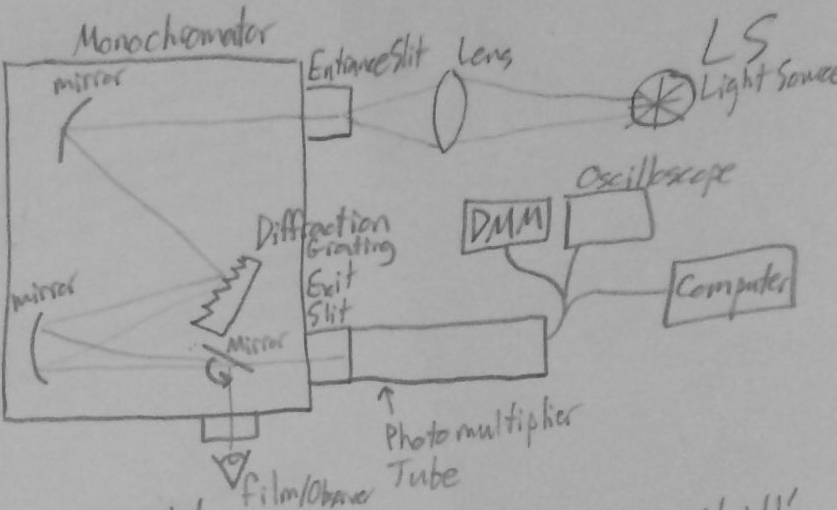
\includegraphics[scale = 0.2]{ATM1a.jpg}
    \caption{}
    \label{fig:my_label}
\end{figure}
    Drawn above is a sketch of the path that light takes during this experiment. We will follow this path and detail how the equipment was used. The light is produced using a lamp. Electrons from a power supply are sent from the cathode to the anode of this lamp after they are subject to a certain potential. As the electrons collide with atoms in the lamp, they excite these atoms, causing stimulated absorption and spontaneous emission. The light travels through a lens, where it is focused onto the entrance slit of a meter monochromator, a device that allows you to scan individual wavelengths of a light spectrum. We adjusted the slit width, the lens position, and the hydrogen lamp's orientation so that they were aligned and so the most light could enter the monochromator. The light enters the monochromator and is reflected by a mirror onto a diffraction grating, which serves to separate the light into its individual wavelengths by reflecting the light of certain wavelengths at different angles. Repetitive arrays of obstacles make up the grating and give it its dispersive effect, causing light of different wavelengths to travel different paths, which in turn will cause them to interfere differently on detectors, generating the spectrum. After the light reflects off of the diffraction grating, it is focused by yet another mirror and then can travel two possible paths, as set by the experimenter. 
    \\\indent A knob on the top of the monochromator allows you to rotate a mirror in the device that can send the light towards your eye/camera or towards an exit slit that leads to a photomultiplier tube. The photomultiplier tube functions by putting out a voltage signal proportional to the amount of light that falls on it, with some limitations for various wavelengths that are specified in its user manual. The photomultiplier essentially applies an electric field along its axis, and consists of a series of metallic plates with loosely bound electrons. When light strikes these plates, electrons are let loose, accelerated, and then they can smash into electrons on subsequent plates, giving way to a cascading effect where the collision of a few electrons leads to the movement of many more, generating a current and a signal. Adjusting the voltage of the attached Fluke voltage supply allows you to generate larger signal outputs. This electrical signal is either fed into an oscilloscope, a DMM, or the data acquisition card of a computer for digital input. Another knob, called the wave knob, at the front side of the monochromator allows you to manually scan wavelengths of the spectrum by rotating the angle of the diffraction grating to illuminate different emission lines. There is also a speed knob, which you can engage to have a step motor perform the rotation at a specified fixed rate. 
    \\\indent My partner and I hooked up the electrical equipment so that the photomultiplier's output could be fed to the three measurement devices, and then we manually scanned wavelengths until we generated a large signal in the oscilloscope. The maximum amplitude signal relative to nearby scanning positions is close to our peak wavelength in that scanning region. My partner and I then manually set a low wavelength using the wave knob, then turned on speed scanning at a speed N = 20 while operating a computer LabView program that captures the amplitude of the signal as we scan past various wavelengths of the light spectrum. We did a slow high-resolution scan of each light spectrum to capture well defined light spectrums, as seen below for mercury and hydrogen. First, we put in a mercury lamp as our light source and scanned it to serve as a calibration for the hydrogen light source, which we scanned next. We recorded the mercury and hydrogen spectrums below, and then output the data to conduct further analysis on it, such as measuring wavelengths or computing the Rydberg constant.
    
    %hydrogen vs mercury lamp
    \subsection{Zeeman Effect}
    \begin{figure}[H]
    \centering
    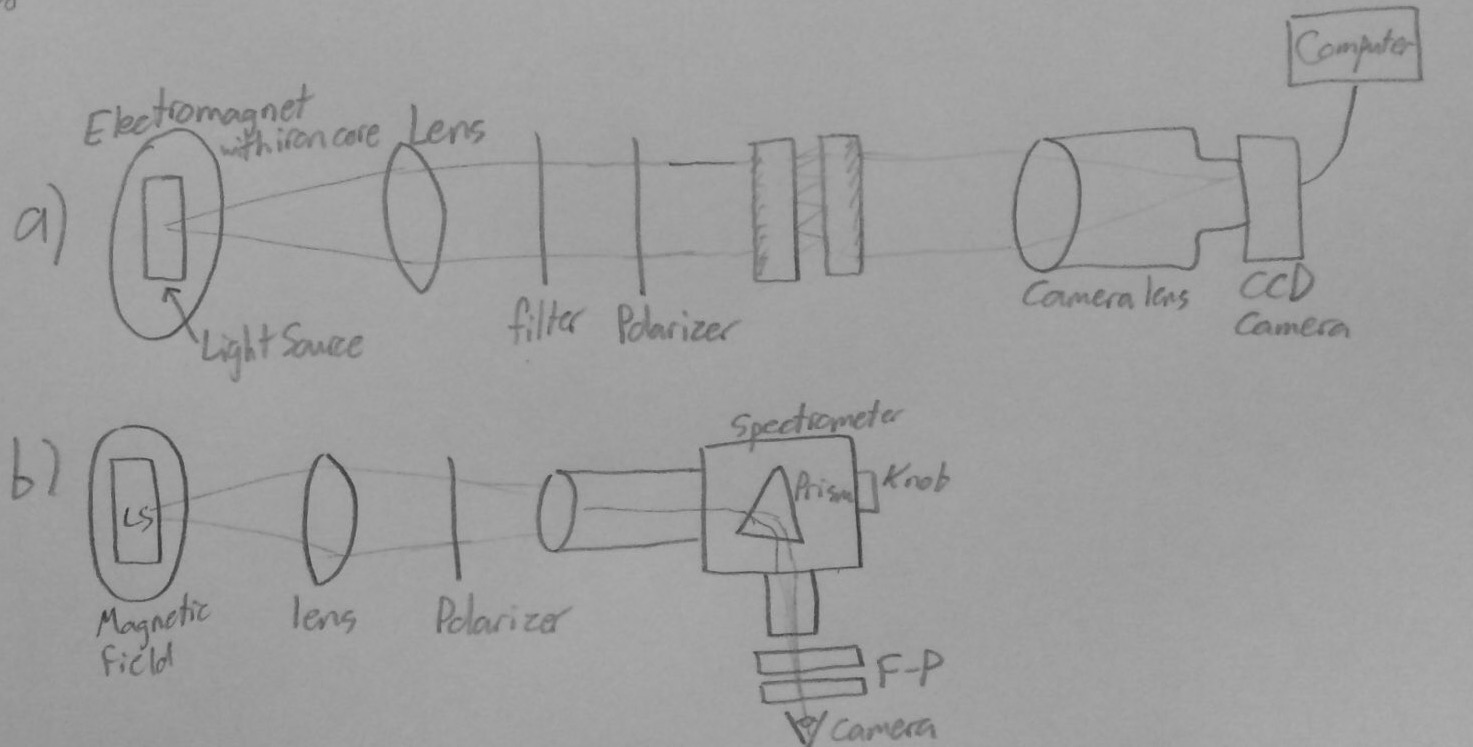
\includegraphics[scale = 0.2]{ATM1e.jpg}
    \caption{}
    \label{fig:my_label}
\end{figure}
    Once again, we have drawn the light path in the above figure. We are going to turn on a helium light source after turning on cooling air (so that the lamp doesn't get too hot and break). The black transformer and the wooden box marked "HIGH VOLTAGE" that orinally came with the set up were destroyed by a previous lab group, so the hydrogen lamp was taken apart and modified to serve as a replacement power supply to the helium lamp. A helium discharge tube (functions the same way as the hydrogen lamp) is placed inside a coiled electromagnet with an iron core such that the current travelling through the coils will generate a uniform magnetic field along the coils' cylindrical axis. 
    \\\indent Before we turn on the light source, we made sure that all of our optical elements and measurement equipment were aligned (perpendicular to the magnetic field) and set up properly. For our first experimental setup of the Zeeman effect (above figure part a), we first set up a lens to collimate the light and get as much of it into the interferometer. A red filter was set up to the right of the lens to pass red light through to eliminate interference patterns from other wavelength light. We then set up a polarizer that would allow you to rotate the polarization direction such that either $\pi$-components or $\sigma$-components can be filtered out at a given moment. This will allow you to directly see the Zeeman splittings, because when you rotate the polarizer, the $\pi$ line that coincides with the degenerate lines without a magnetic field will give way to two $\sigma$ lines, equally spaced but opposite in direction from the central $\pi$ lines on the interference fringes. The light passing though the polarizer then enters the Fabry-Perot (FP) interferometer, which as discussed earlier alters the optical path of adjacent wavefronts such that they form interference patterns on a detector. The FP has been chosen in this experiment over a diffraction grating because the FP has a much higher resolution, allowing you to better make out the interference fringes. Once the light passes through all of these optical elements, it passes into a CCD camera that is focused at infinity, and the camera helps magnify and view these fringes. The diffraction image picked up by the camera is displayed real-time on a computer using a program (we are able to save images of these diffraction patterns; for later analysis). My partner and I set up all of the optical elements, aligned them with the light source (perpendicular to the electromagnet's cylindrical axis), turned on the light source, and looked at a real-time display of the diffraction patterns on our computer. We adjusted the position and orientation of the optical elements until our image was as sharply defined as it could be and was bright enough to distinctively see the pattern. We zoomed out and used micrometer adjustment knobs on the FP mount to center our diffraction image. We manually adjusted the lens in the camera and also used the computer to control the CCD.\\\indent To generate the splittings, we must turn on the magnetic field and increase the voltage being fed to it. We turned on a LAMBDA DC Power supply and current limited it to 2 amps to avoid generating excess heat in the coils of the electromagnet (such heat could reduce the current and the field being measured as well as cause the interference fringes splittings to decrease). We increased the DC power to send current to the coils, thereby increasing the magnetic field. With the polarizer in the correct orientation (able to see $\sigma$ components), we increased the magnetic field strength until we began to produce $\sigma$ lines. Before these lines split, they were joined together at various orders, and then we kept increasing the field until the $\sigma$ lines from adjacent orders began to come together and overlap. In this scenario, we say that the Zeeman splittings were about $\Delta n$ = $\frac{1}{2}$ of an order. At this point, all of the diffraction circles were evenly spaced from each other. Another option was to create splittings of about $\frac{1}{4}$ of an order, where we would increase the fields until the $\sigma$ fringes were evenly spaced, but only half the distance to where they overlaped. To take a measurement for a trial, we would set the magnetic field to 0T and then save a picture of the diffraction pattern on the computer. Then we would increase the field to the change of order we would like to measure, and take another picture of the diffraction pattern. We used a gaussmeter to measure the magnetic field at the center of the coils of the electromagnet by placing a probe as close to the iron core as possible. The gaussmeter's probe must first be calibrated by inserting it into a 1000 gauss calibration magnet and adjusting the gaussmeter readings appropriately. We recorded the magnetic field values ten different times by moving the probe around near the iron core and taking the probe in and out of the field, each time taking new measurements. We then decreased the field to 0 gauss, and increased it again to the ideal order of zeeman splittings. We took another picture and recorded ten more magnetic field values. The process was repeated multiple times until enough data was taken. Between each trial, we would make sure not to move the camera (for the upcoming digital analysis), and everytime we manipulated the set up, we would take an initial image of the diffraction fringes before the application of the field. We did this while measuring zeeman splittings for the red energy transition.\\\indent In the above figure part b, we had a new set up where we used a lens to focus the light into a spectrometer, which would split up the light into its spectra using a prism to refract different frequency light at different angles. The bent light travelled out of an exit slit and through a polarizer and FP and into the lens of a camera. Here, we can rotate the prism for filter for the color of Helium we would like to see. In this case, we observed zeeman splittings of red and yellow light and performed the same magnetic field measurements. %why we use fabry perot
    % tomorrow finish then do calc and data analysis on Thursday, PH, YMM if time, Fri- Conclusion or finish data analysis, finish  problem with lens
    

\section{Calculation and Data Analysis}
% error from picture analysis in choosing center of circle and if image position changed
    The data for both lab sections were analyzed using MATLAB, and relavant expressions produced below have their equivalent MATLAB expressions/functions, but are not reproduced to save space. MATLAB code can be produced upon request:
    \subsection{Balmer Series}
    The raw data we got from using the LabView program and the monochromator to wavelength scan the spectrums of mercury and hydrogen, which yielded the following (wavelength vs signal) data:
    \begin{figure}[H]
    \centering
    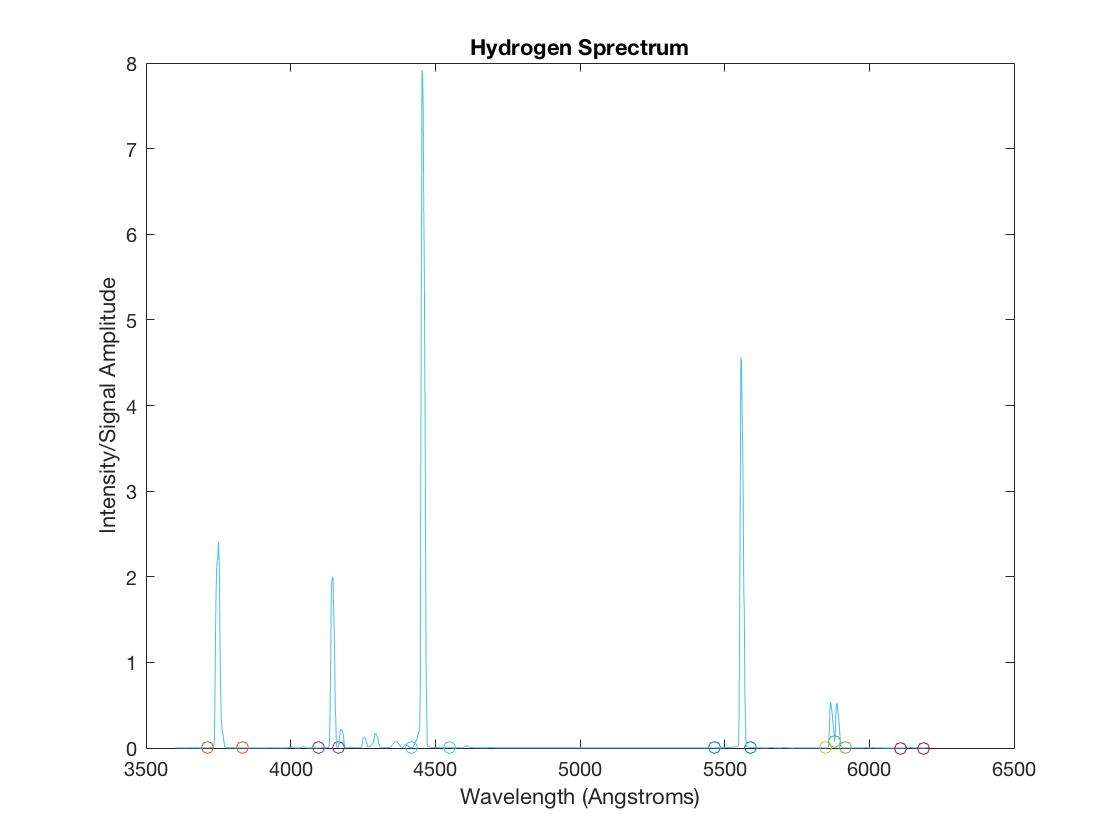
\includegraphics[scale = 0.2]{ATMf.jpg}
    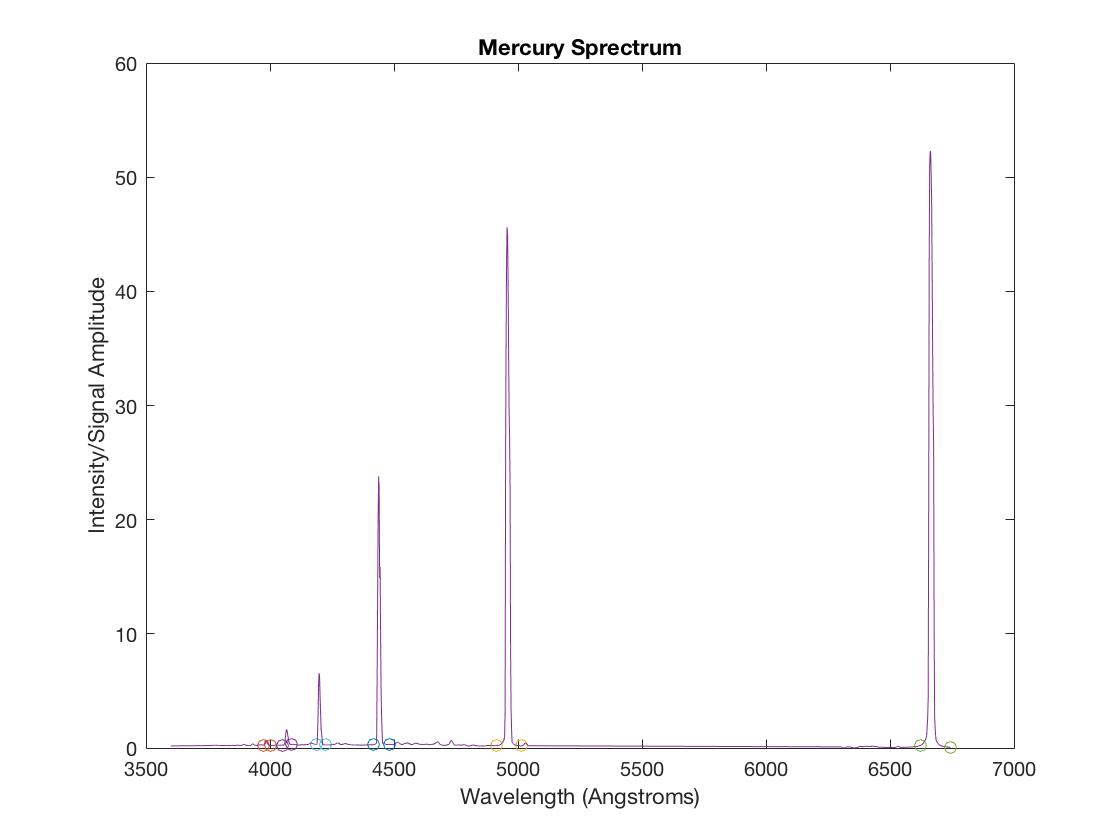
\includegraphics[scale = 0.2]{ATMg.jpg}
    \caption{}
    \label{fig:my_label}
\end{figure}
    
    Using MATLAB, we removed the constant offset and found the peaks in the spectral data for both the hydrogen and mercury spectrum by fitting gaussian curves to datapoints around local maxima. The local maxima were all selected on the criteria that their peak signals were above certain threshold and the maxima were not accidentally too closely horizontally spaced (maxima had to be a greater than certain distance from each other). This removed any unnecessary peaks. Local minima were found around each spike in the spectral signal, and specral data was fitted in the interval between the closest two minima to a peak. Here is the model we fit to: f(x) =  a*exp(-((x-$\lambda$)/c)\^{}2). The wavelength of the peak was found ($\lambda$), along with the error of this wavelength ($\Delta \lambda$), which we took to be half of the range of the 95$\%$ confidence interval of the fit parameter b. We also checked to see if the gaussian fit produced accurately modelled the data, so we calculated correlational reduced $R^{2}$ values (essentially measures the sum of the residuals squared of the data and normalizes it) for each gaussian fit. An $R^{2}$ value of 1 would indicate that we have chosen a good model to represent the data, and an $R^{2}$ value of 0 would mean that we have chosen a bad model. In the table below, we find the wavelengths of hydrogen and mercury measured, and their associated errors as well as their goodness of fit $R^{2}$ values. Also, the expected mercury in air wavelengths are displayed:
    FIGURE
    
    Next, we calculated a weighted least-squares best fit line between the measured mercury wavelength values and the expected mercury wavelength values to serve as a calibration reference to convert the measured hydrogen wavelengths into the actual wavelengths we measured in air. This eliminates almost all biases introduced by the data acquisition element on the computer and any issues with the monochromator as it rotates the diffraction grating (and other speed and timing errors in measurement). The weights we used in the mercury calibration fit is:
    \begin{equation}
        w_i = \frac{1}{\Delta b_i^2}
    \end{equation}
    where $w_i$ is the ith weight of the data set and $\Delta b_i$ is the error in the wavelength measurement. We also found a goodness of fit reduced chi-squared value to be 0.5097 using the formula:
    \begin{equation}
        \tilde{\chi}^2 = \frac{\sum_i \frac{(\lambda_{HgOberved_i} - \lambda_{HgAirCorrect_i})}{\Delta b_i^2}}{df}
    \end{equation}
    where df = 4, which is the degrees of freedom of the data set.
    This indicated a reasonably good model. The discovered b best fit line (y = mx + b) is:
    \begin{equation}
        \lambda_{airCorrect} = 1.0001 \lambda_{measured} -99.0710 \buildrel _\circ \over {\mathrm{A}}
    \end{equation}
    The error in the slope and intercept are $\Delta m = 2.1298*10^{-04}$ and $\Delta b = 1.0603 \buildrel _\circ \over {\mathrm{A}}$ using formulas \cite{err}: 
    \begin{equation}
        \Delta b = \sqrt{\frac{\sum_i w_i*x_i^2}{\delta}}
    \end{equation}
    \begin{equation}
        \Delta m = \frac{\sum_i w_i}{\Delta}
    \end{equation}\begin{equation}
        \Delta = (\sum_i w_i)*(\sum_i w_i*x_i^2)-(\sum_i w_i*x_i)^2
    \end{equation} Below is a graphical display of this line and its errorbars along with actual plotted data points.
    \begin{figure}[H]
    \centering
    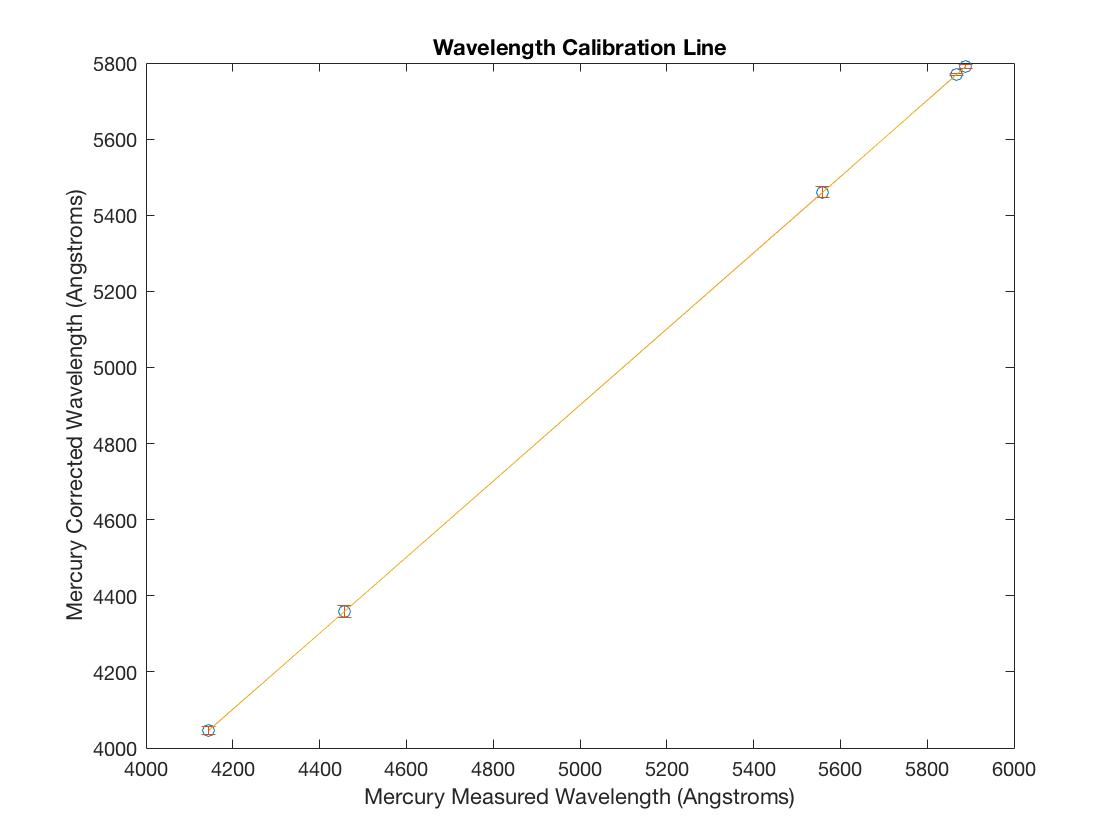
\includegraphics[scale = 0.2]{ATMi.jpg}
    \caption{}
    \label{fig:my_label}
\end{figure}
    \\\indent We then plug in our measured values for hydrogen wavelengths into the above function and then output our corrected air wavelengths $\lambda_H$. The errors on the hydrogen wavelengths were also modified, using propagation of errors from our calibration fit for each hydrogen wavelength error datapoint:
    \begin{equation}
        \Delta \lambda_{hydrogenAirCorrected} = \sqrt{(\lambda_H*\Delta m)^2 + m^2 + \Delta b ^2}
    \end{equation}
    We then converted the hydrogen air wavelengths into vacuum wavelengths ($\lambda_{Hv}$) utilizing the relationship from refractive index n:
    \begin{equation}
        \lambda_{hydrogenAirCorrected} = \frac{\lambda_{Hv}}{n} = \frac{\lambda_{Hv}}{1 + 6432.8*10^{-8} + \frac{2949810}{146*10^8 - (1/\lambda_{Hv})^2} + \frac{25540}{41*10^8 - (1/\lambda_{Hv})^2}}
    \end{equation}
    and solving for each $\lambda_{Hv}$ for each data point, which we did via a numerical solver in MATLAB. The errors on the hydrogen wavelengths were again corrected to anything below a second order correction. Thus we neglected $\lambda_{Hv}^(-2)$ terms in our error correction.
    \begin{equation}
        \Delta \lambda_{Hv} = \Delta \lambda_{hydrogenAirCorrected} * n =\Delta \lambda_{hydrogenAirCorrected} * (1 + 6432.8*10^{-8} + \frac{2949810}{146*10^8} + \frac{25540}{41*10^8})
    \end{equation}
    With corrections in place, the original measured hydrogen values, corrected ones due to the mercury calibration, and the air to vacuum corrected values are displayed below with their associated uncertainties and n value. The n value is not the same as the refective index above, it represents the quantum number that is being transitioned from in the Balmer Series:
   
    \scalebox{0.6}{
\centering
\caption{}
\label{my-label}

\begin{tabular}{llllll}
\textbf{$R^{2}$ Mercury} & \textbf{Expected Mercury Wavelength} & \textbf{Wavelength Mercury Found} & \textbf{Error Mercury} &  &  \\
\textbf{} & \textbf{Angstroms} & \textbf{Angstroms} & \textbf{Angstroms} &  &  \\
0.9796 & 4046.6 & 4144.9 & 0.3036 &  &  \\
0.9828 & 4358.3 & 4457.1 & 0.2557 &  &  \\
0.9793 & 5460.7 & 5559.1 & 0.2558 &  &  \\
0.9783 & 5769.6 & 5868.5 & 0.749 &  &  \\
0.9322 & 5790.7 & 5889.1 & 0.4609 &  &  \\
\textbf{Wavelength Hydrogen} & \textbf{Hydrogen Vacuum Air Wavelengths} & \textbf{Error Hydrogen} & \textbf{n-value} & \textbf{Expected Hydrogen Wavelength} & \textbf{$R^2$ Hydrogen} \\
\textbf{Angstroms} & \textbf{Angstroms} & \textbf{Angstroms} & \textbf{} & \textbf{Angstroms} &  \\
3984.8 & 3887.2 & 2.177 & 8 & 3889 & 0.7194 \\
4067.8 & 3970.2 & 1.644 & 7 & 3970.1 & 0.8759 \\
4198.8 & 4101.3 & 1.4401 & 6 & 4101.7 & 0.9699 \\
4439.2 & 4341.8 & 1.4653 & 5 & 4340.5 & 0.9708 \\
4958.2 & 4861.1 & 1.5653 & 4 & 4861.3 & 0.9609 \\
6665.2 & 6568.7 & 1.8259 & 3 & 6562.7 & 0.9641
\end{tabular}
}


    We calculate $\frac{1}{\lambda_{Hv}}$ with its associated error $Err(\frac{1}{\lambda}) = \frac{\Delta \lambda_{Hv}}{\lambda_{Hv}^2}$ and its corresponding $\frac{1}{n^2}$ value for the found hydrogen wavelengths. Using weights:
    \begin{equation}
        w_i = \frac{1}{Err(\frac{1}{\lambda})_i^2}
    \end{equation}
    and $\frac{1}{\lambda_{Hv}}$ and $\frac{1}{n^2}$, which are displayed below:
    \begin{figure}[H]
    \centering
    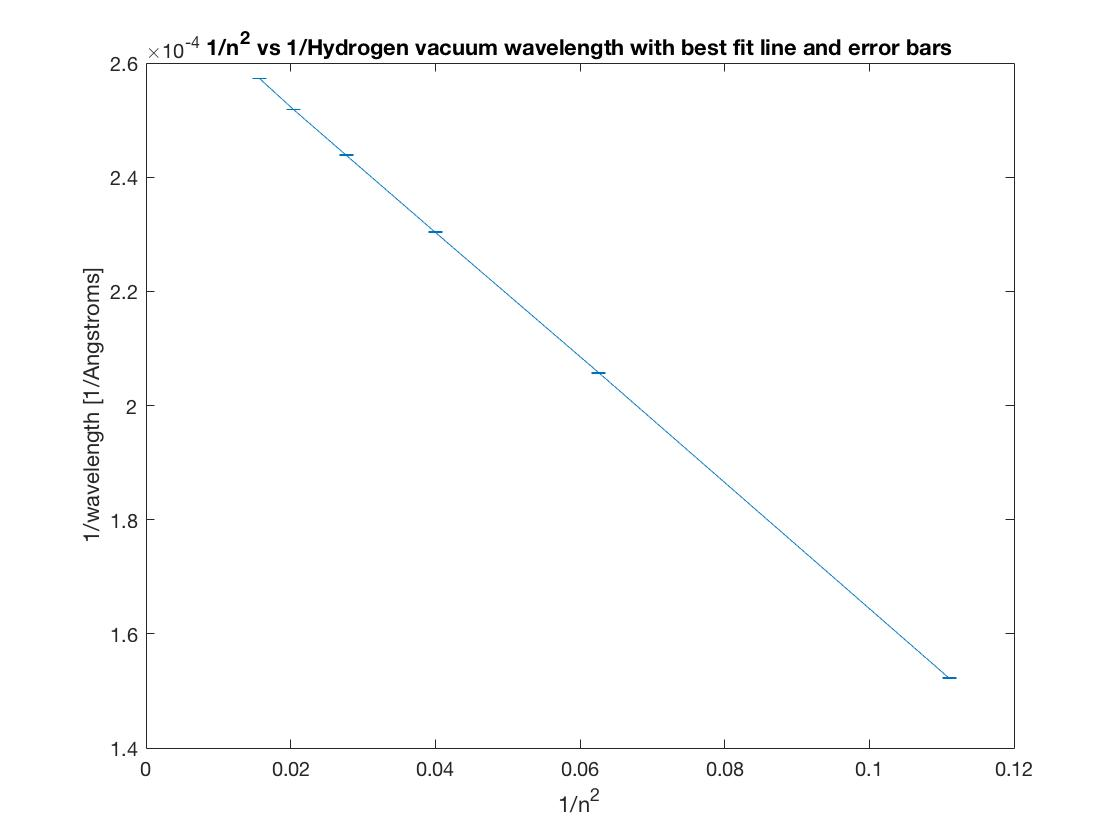
\includegraphics[scale = 0.2]{ATMj.jpg}
    \caption{}
    \label{fig:my_label}
\end{figure} and we using a weighted least squares regression line fit, we find the line of best fit for $\frac{1}{n^2}$ vs. $\frac{1}{\lambda_{Hv}}$ (form y = mx + b) to be:
    \begin{equation}
        \frac{1}{\lambda} = -1.099723*10^{-03}*\frac{1}{n^2} + 2.7439*10^{-04} \buildrel _\circ \over {\mathrm{A}}^{-1}
    \end{equation}
    and associated weighted errors for slope m and intercept b (eq.(29,28)) are calculated to be -$1.3*10^{-06} \buildrel _\circ \over {\mathrm{A}}^{-1}$ and $4.71*10^{-08} \buildrel _\circ \over {\mathrm{A}}^{-1}$ respectively. The slope of the best fit line is -R, the Ryberg constant, and the intercept is series limit R/4. The accepted values for R is $0.001099 \pm 4.71*10^{-08} \buildrel _\circ \over {\mathrm{A}}^{-1}$ and $2.74*10^{-4}\pm 1.3*10^{-06} \buildrel _\circ \over {\mathrm{A}}^{-1}$. Both of these values lie outside of the error interval generated for our found R and R/4. However, the relative error between experimental and theoretical for values of R and R/4 are 0.2142$\%$ and 0.0179$\%$ respectively. The reduced chi-square value calculated for this fit is 0.7789, which means that the best fit is a reasonable strong model.
    
    \subsection{Zeeman Effect}
    Each experimental set up was titled differently and labelled according to the color of incoming light, whether a quarter order or half order change was expected due to the spacing between the $\sigma$ components, if the trials from the set up should be kept or thrown out, and the number of times trials were taken using that setup. For instance, the name "Red3halfspecGood" means that red was observed, a prism spectrometer was used to take the data, the trials were to be included in the final analysis (good vs bad), we were observing half an order splittings, and this was the third set up using red light. Typically for a given set up, two trials were conducted (raw data: three images of the diffraction fringes- two of the splittings and one of no splittings- and two sets of ten magnetic field measurements). I will now go through the steps of analysing two trials from one experimental set up and then show how data between set ups were combined to produce meaningful data:
    \begin{enumerate}
        \item No split image is loaded, and then adjusted to bring out highest contrast through image adjust and histogram equalizer image processing techniques. The center of the diffraction fringes is found with help from user input. A line is drawn radially outward from the center of the image and a point is found on that line that lies outside of the most inner circle of the pattern to reduce noisiness in the dataset. An intensity profile is found along the line, that is, the image is cut on its side and a plot of distance from the center of the fringes versus the intensity of light or signal is plotted and recorded. We assume that this intensity profile is the same radially in all directions.\begin{figure}[H]
    \centering
    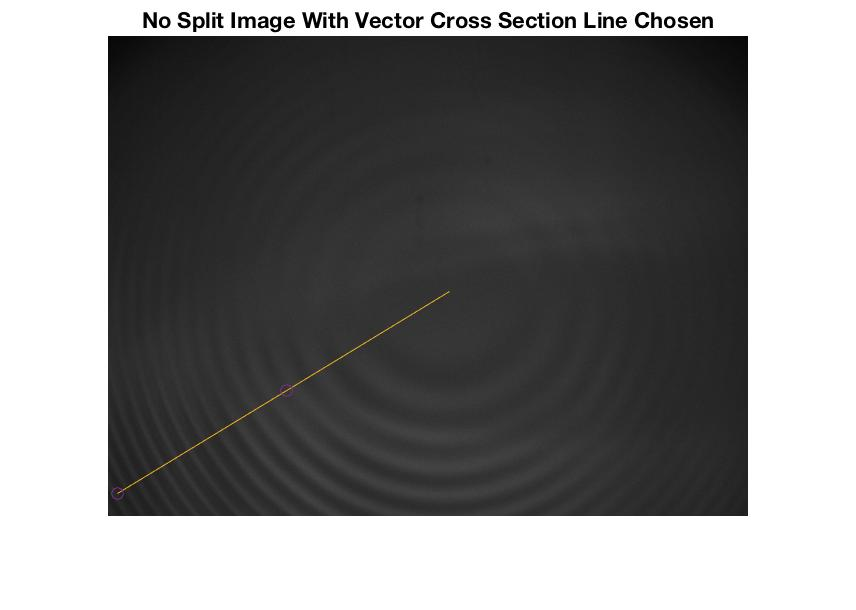
\includegraphics[scale = 0.2]{ATMk.jpg}
    \caption{}
    \label{fig:my_label}
\end{figure}
        \item We find intensity profiles for the other trials in the setup (two intensity profiles for the split images). We made sure in taking data for our lab not to change anything about the experimental set up, so the line that the intensity profile is taken using is the exact same line for all three photos per set up. For each intensity profile, we generate en envelope function that connects the valleys/local minima of the intensity profile. The values of the envelope are subtracted from the intensity values to shift the intensity profile towards zero on the vertical axis so that better fits can be produced. The three intensity profiles are plotted together, with a smoothing filter applied to each for ease of viewing. Note how $\pi$ components/degenerate lines and $\sigma$ components are separated differently. If there are two trials for a set up, there will be two $\sigma$ component lines that roughly overlap. \begin{figure}[H]
    \centering
    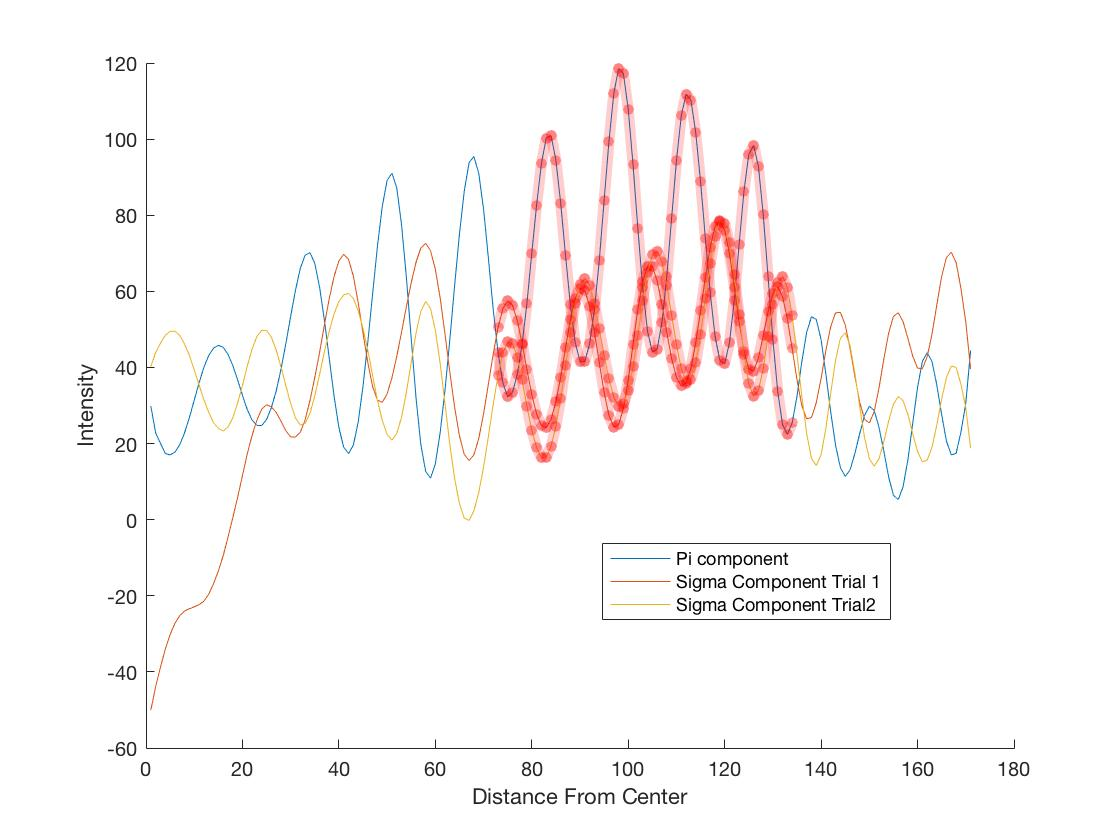
\includegraphics[scale = 0.2]{ATMl.jpg}
    \caption{}
    \label{fig:my_label}
\end{figure}
        \item For each intensity profile, the user chooses a distance value on this graph for which an interval spanning exactly five valleys of the smoothed intensity data (inverval over the next five local minima) is found. This interval spans ten local minima for trials that are from split images and expecting order changes of one quarter and five minima for any other condition (above figure, interval is highlighted in red). 
        \item A series of four gaussian curves are fit to data points within the intensity curve interval using the fit model:
        \begin{equation}
            f(x) = \sum_i G(x) =  a1*exp(-((x-b1)/c1)^2) + a2*exp(-((x-b2)/c2)^2) + 
              a3*exp(-((x-b3)/c3)^2) + a4*exp(-((x-b4)/c4)^2)
        \end{equation}
        for which we find b1, b2, b3, b4, which are the location of the intensity peaks (center of fringes) (from the center of the image) with associated errors $\Delta b1, \Delta b2, \Delta b3, \Delta b4$ found from half of the range of the 95$\%$ confidence interval of the fit parameter utilizing the fit algorithm.
        \begin{figure}[H]
    \centering
    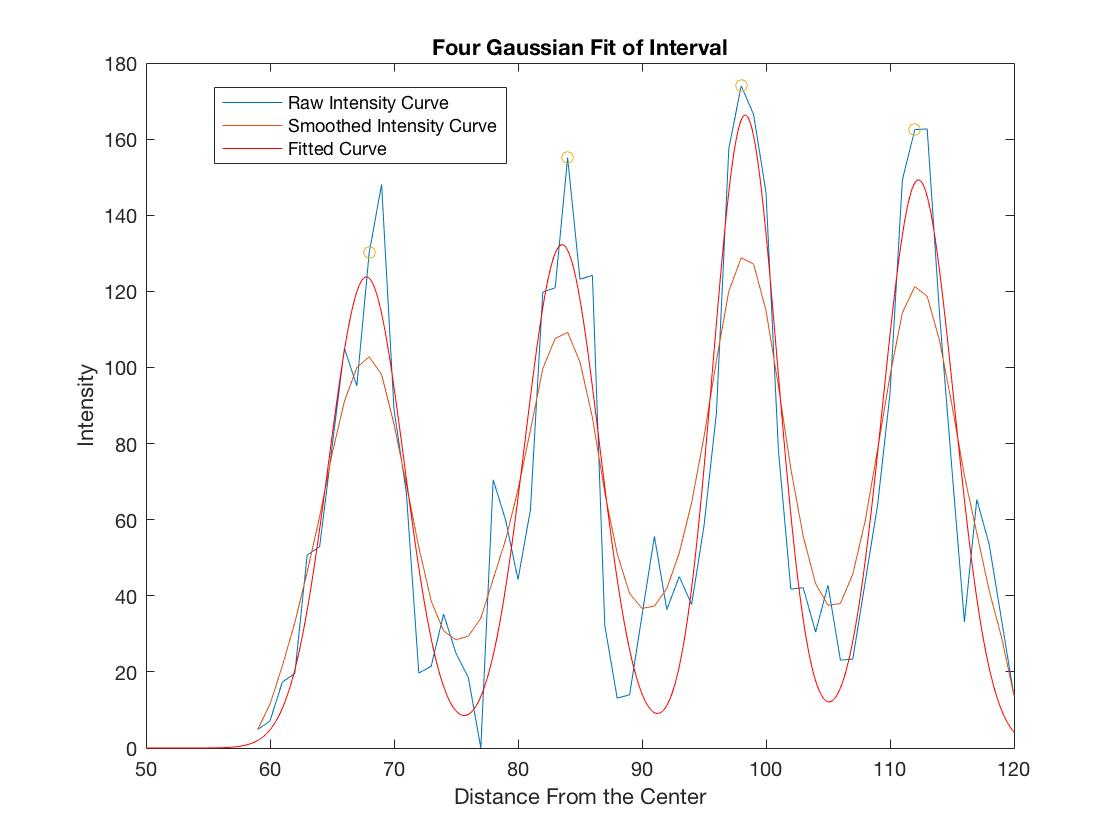
\includegraphics[scale = 0.2]{ATMm.jpg}
    \caption{}
    \label{fig:my_label}
\end{figure}
Adjusted (using degrees of freedom) correlational $R^2$ values are calculated for each model fit, and a model will only be accepted as valid as long as all $R^2$ values found from fitting the no split intensity profile and intensity profiles of two images with splittings are above 70 $\%$, demonstrating that the model that was fit to is a reasonable description for the data. If this $R^2$ value was not passed for setups described as "Good" and "Red", then all previous steps were repeated until a better intensity cross section or interval was chosen. The "Bad" and "Yellow" data was still fit, but $R^2$ values under 70 $\%$ were acceptable because our analysis is focused on the good red zeeman splittings. In the case that a quarter of an order is being analyzed, eight gaussian curves are fit to the interval because there are twice as many peaks for the $\sigma$ components are there are for $\pi$ components.
        \item The distances between adjacent peaks are found ($d_j$, j and i are indices):
        \begin{equation}
            d_j = b_{i+1} - b_i
        \end{equation}
        and error:
        \begin{equation}
            \Delta d_j = \sqrt{\Delta b_{i+1}^2 +\Delta b_i^2}
        \end{equation}
        and we wind up with three distances per trial. In the case that a quarter order splitting is being analyzed, we find six distances but we reduce this number to three by generating weighted averages (weights $w_j = \frac{1}{\Delta d_j^2}$) between consecutive distance values (we take j=1,2 ; j=3,4; and j=5,6 distances as our distance pairs being averaged) \cite{err}:
        \begin{equation}
            d_{j,j+1} = \frac{\sum_j^{j+1} w_j d_j}{w_j}
        \end{equation}
        with error:
        \begin{equation}
            \Delta d_{j,j+1} = \frac{1}{\sqrt{\sum_j^{j+1} w_j}}
        \end{equation}
        because the six distance points collapses into three, we can give the distances their original indices of j=1, 2, 3 instead of using $d_{j,j+1}$, and the error is as such as well. The rest of the analysis method for quarter of an order splitting versus half order splitting are the same.
        \item We denote distance values between fringes from the no split image to be $D_i$ for i = 1, 2, 3 and distance values for a split image to be $d_i$. We only focus on comparing one split image/interference pattern to one nonsplit image/interference pattern, but we can extend this analysis to include another trial for a given experimental setup. The given trial has ten magnetic field measurements. We can say that the B-field for a trial is $B \pm \Delta B$, where B is actually the mean B field and $\Delta B$ is the standard deviation of the B field measurements. Because we recorded a different value for the magnetic field at different points, we presume this to be a measurement error. 
        \item The change of order, or fraction of the order difference between subsequent interference fringes of ($\Delta n$ = 1 for $\pi$ components or degenerate lines but is variable for $\sigma$ components and scales with the magnetic field). We increased the magnetic field such that the change in order between fringes is either $\Delta n =$ 0.5 or 0.25 from the $\pi$ component line for $\sigma$ components. We consider three distance points for the split and no split intensity profiles to find this value. Because of naming conventions for errors, we rename the change in order to $\delta n$. We find that, for distance j between the two images:
        \begin{equation}
            \delta n_j = \frac{d_j}{D_j}*0.5
        \end{equation}
        The 0.5 value stems from the assumption that the distance between the $\pi$/degenerate line to the $\sigma$ line is half the distance between two $\sigma$ components that are split off from a $\pi$ component. And the associated error using error propagation:
        \begin{equation}
            \Delta \delta n_j = \frac{1}{2*D_j}*\sqrt{\Delta d_j^2 + (\frac{d_j * \Delta D_j}{D_j})^2}
        \end{equation}
        \item From here, we want to find the ratio of energy level splittings to the magnetic field strength. We will call this $r_j$ for the jth splitting distances being analyzed. We find that:
        \begin{equation}
            r_j = \frac{\Delta \sigma}{B} = \frac{\delta n}{2t*B}
        \end{equation}
        where $\Delta \sigma$ and t have been defined in the theory section of the lab, and we are given t = 8.11mm. Error $\Delta r_j$ is: % 1/(2*0.811*Bmean(i))*(orderErr.^2+(Bstd(i)*orderChange./Bmean(i)).^2).^(1/2)
        \begin{equation}
            \Delta r_j = \frac{\sqrt{\Delta \delta n_j^2 + (\frac{\Delta B * \delta n}{B})^2}}{2*t*B}
        \end{equation}
        \item And finally, we can calculate the value for the bohr magneton $\mu_B$. Plugging in S = 0, L = 1, and J = 1 into equation 21 to get $g_J$ = 1 and considering a splitting from an energy transition where $\Delta m_J = 1$ (slight change from j to J to avoid confusion in indexing), and we see that:
        \begin{equation}
            \mu_{B_j} = \frac{hc\delta n}{2t*g_J*\Delta m_J*B} = hc * r_j
        \end{equation}
        where hc equals $1.98644568*10^{-25}$ Joule-meters. And the error:
        \begin{equation}
            \Delta \mu_{B_j} = hc \Delta r_j
        \end{equation}
        \item To find the final $\delta n, r_j,$ and $\mu_B$ values for a given trial, we use the weighted average formula between values for j= 1, 2, 3. The weighted average for a given calculated value (substitute either $\delta n, r_j,$ or $\mu_B$ into this equation) for some calculated weighted average $\bar{x}$:
        \begin{equation}
            \bar{x} = \frac{\sum_j w_j x_j}{w_j}
        \end{equation}
        with error:
        \begin{equation}
            \Delta \bar{x} = \frac{1}{\sqrt{\sum_j w_j}}
        \end{equation}
        where $w_j = \frac{1}{\Delta x_j}$ for j = 1, 2 ,3.
    \end{enumerate}
    You can repeat the previous steps for any other trial/split image for each experimental setup. However, we changed experimental setups over the course of the experiment. Displayed below is a table of all of the different setups (analyses), their run/trial/split image, and then measured and calculated magnetic field means, the order change of the splitting, the energy splitting ratio with the magnetic field, and the calculated bohr magneton with errors calculated for each. 
    \scalebox{0.6}{
\centering
\caption{}
\label{my-label}
\begin{tabular}{llllll}
\textbf{Analysis} & \textbf{Red1halfGood} & \textbf{Red1halfGood} & \textbf{Red2quarterGood} & \textbf{Red3halfspecGood} & \textbf{Red3halfspecGood} \\ \cline{2-6} 
\multicolumn{1}{l|}{\textbf{Run}} & 1 & 2 & 1 & 1 & 2 \\
\multicolumn{1}{l|}{\textbf{Mean Magnetic Field (Gauss)}} & 5280 & 5210 & 2710 & 6880 & 6770 \\
\multicolumn{1}{l|}{\textbf{B Error (Gauss)}} & 198.8852 & 159.513 & 119.721 & 234.757 & 271.006 \\
\multicolumn{1}{l|}{\textbf{Order Change}} & 0.5003 & 0.4991 & 0.26424 & 0.4531 & 0.4563 \\
\multicolumn{1}{l|}{\textbf{Order Change Error}} & 0.02208 & 0.0216 & 0.00646 & 0.0144 & 0.01463 \\
\multicolumn{1}{l|}{\textbf{Splitting Ratio (cm^-1 / Gauss)}} & 5.84E-05 & 5.91E-05 & 6.01E-05 & 4.08E-05 & 4.17E-05 \\
\multicolumn{1}{l|}{\textbf{Splitting Ratio Error(cm^-1 / Gauss)}} & 2.88E-06 & 2.78E-06 & 2.12E-06 & 1.55E-06 & 1.67E-06 \\
\multicolumn{1}{l|}{\textbf{Bohr Magneton (J/T)'}} & 1.16E-23 & 1.17E-23 & 1.19E-23 & 8.10E-24 & 8.28E-24 \\
\multicolumn{1}{l|}{\textbf{Bohr Magneton Error (J/T)'}} & 5.71E-25 & 5.52E-25 & 4.22E-25 & 3.08E-25 & 3.31E-25 \\ \hline
\multicolumn{1}{l|}{\textbf{Analysis}} & \textbf{Red2quarterBad} & \textbf{Red2quarterBad} & \textbf{Red2quarterBad} & \textbf{Red2quarterBad} & \textbf{Yellow1halfspecGood} \\ \cline{2-6} 
\multicolumn{1}{l|}{\textbf{Run}} & 1 & 2 & 1 & 2 & 1 \\
\multicolumn{1}{l|}{\textbf{Mean Magnetic Field (Gauss)}} & 7460 & 7580 & 7460 & 7580 & 6250 \\
\multicolumn{1}{l|}{\textbf{B Error (Gauss)}} & 353.396 & 304.776 & 353.396 & 304.7764 & 206.827 \\
\multicolumn{1}{l|}{\textbf{Order Change}} & 0.2425 & 0.4488 & 0.45827 & 0.4441 & 0.2361 \\
\multicolumn{1}{l|}{\textbf{Order Change Error}} & 3998.077 & 439.476 & 0.02087 & 0.09231 & 0.00696 \\
\multicolumn{1}{l|}{\textbf{Splitting Ratio (cm^-1 / Gauss)}} & 2.00E-05 & 3.65E-05 & 3.79E-05 & 3.61E-05 & 2.01E-05 \\
\multicolumn{1}{l|}{\textbf{Splitting Ratio Error(cm^-1 / Gauss)}} & 0.33041 & 0.03574 & 2.49E-06 & 7.65E-06 & 1.04E-06 \\
\multicolumn{1}{l|}{\textbf{Bohr Magneton (J/T)'}} & 3.98E-24 & 7.25E-24 & 7.52E-24 & 7.18E-24 & 4.00E-24 \\
\multicolumn{1}{l|}{\textbf{Bohr Magneton Error (J/T)'}} & 6.56E-20 & 7.10E-21 & 4.94E-25 & 1.52E-24 & 2.07E-25 \\ \hline
\multicolumn{1}{l|}{\textbf{Analysis}} & \textbf{Yellow1halfspecGood} & \textbf{Yellow1quarterBad} & \multicolumn{1}{l|}{\textbf{Yellow1quarterBad}} & \textbf{Final Analysis} &  \\ \cline{2-4}
\multicolumn{1}{l|}{\textbf{Run}} & 2 & 1 & \multicolumn{1}{l|}{2} & \textbf{Final Energy Split Ratio [cm-1/gauss]} &  \\
\multicolumn{1}{l|}{\textbf{Mean Magnetic Field (Gauss)}} & 7170 & 6180 & \multicolumn{1}{l|}{6890} & 5.0684 * 10^{-5} &  \\
\multicolumn{1}{l|}{\textbf{B Error (Gauss)}} & 266.87 & 376.533 & \multicolumn{1}{l|}{580.1340} & \textbf{Ratio Error} &  \\
\multicolumn{1}{l|}{\textbf{Order Change}} & 0.3833 & 0.4200 & \multicolumn{1}{l|}{0.4380} & 1.06078*10^{-6} &  \\
\multicolumn{1}{l|}{\textbf{Order Change Error}} & 0.00654 & 0.255 & \multicolumn{1}{l|}{0.003147} & \textbf{Bohr Magneton} &  \\
\multicolumn{1}{l|}{\textbf{Splitting Ratio (cm^-1 / Gauss)}} & 3.25E-05 & 4.19E-05 & \multicolumn{1}{l|}{3.76E-05} & 1.00501E-23 &  \\
\multicolumn{1}{l|}{\textbf{Splitting Ratio Error(cm^-1 / Gauss)}} & 1.34E-06 & 2.56E-05 & \multicolumn{1}{l|}{2.27E-06} & \textbf{Error Final J/T} &  \\
\multicolumn{1}{l|}{\textbf{Bohr Magneton (J/T)'}} & 6.45E-24 & 8.32E-24 & \multicolumn{1}{l|}{7.47E-24} & 2.10792E-25 &  \\
\textbf{Bohr Magneton Error (J/T)'} & 2.66E-25 & 5.09E-24 & 4.51E-25 &  & 
\end{tabular}
}
    The energy split ratios and bohr magneton for every "Good" and "Red" trial were combined together to form our final values for the measured energy split ratios and bohr magneton. Once again, the weighted averages of eq.(47,48) were utilized. This time with k being the trial number when considering the totality of "Good" and "Red" trials. The weights for each good, read trial were $\frac{1}{\Delta \bar{x_k}^2}$ for either the ratio or the bohr magneton for each trial. So performing this calculation, we find that the final value of the energy splitting and bohr magneton are 
    r = $5.0684*10^{-5} \pm 1.06^{-6} \frac{cm^{-1}}{gauss}$ and $\mu_B = 1.00501*10^{-23} \pm 2.11^{-24} \frac{J}{T}$. 
    The empirical value for the bohr magneton is $9.274*10^{-24} \frac{J}{T}$, and we see that this is below the empirical error low bound of the measured value, which is $9.83928*10^{-24} \frac{J}{T}$. The relative error between the experimental and theoretical values of the bohr magneton is about an 8.37$\%$ error.
    
\section{Conclusion}
    We have experimented on two very profound concepts in domain of physics, the balmer series and the Zeeman effect. Both experiments are very quantum mechanical in nature. \\\indent We plotted the spectrums of mercury and hydrogen in order to deduce the peak wavelengths of evergy transitions of the Balmer Series (n $\>$ 2 state down to the n=2 state). By plotting $\frac{1}{n^2}$ versus $\frac{1}{\lambda}$, we found that the actual Rydberg constant R and series limit $\frac{R}{4}$ were outside the experimental bounds of the measured values ($1.099723*10^{-03} \pm 1.335371*10^{-06} \buildrel _\circ \over {\mathrm{A}}^{-1}$ and $2.7439*10^{-04} \pm 4.719338*10^{-08} \buildrel _\circ \over {\mathrm{A}}^{-1}$ respectively). Even though the relative error is off by a small percentage, very precise model fits kept the error low enough for there to be a lack of agreement between experimental and theoretical values.
    \\\indent We passed light from a helium light source through a filter, polarizer, FP interferometer, and lens towards a camera in order to take pictures of interference fringes that result from the behaviors of light waves and differences in path lengths at a boundary. We then turned on a magnetic field until these fringes split apart into $\sigma$ components, and measured the distance between them and compared those values to the distance between $\pi$/degenerate fringes in order to find the amount of energy splitting that was taking place due to the Zeeman effect, the ratio of the energy splitting to the magnetic field was found to be $5.0684*10^{-5} \pm 1.06^{-6} \frac{cm^{-1}}{gauss}$. We could then use those values to find a measurement for the bohr magneton, a fundamental unit of magnetic moment, which we found to be equal to be $\mu_B = 1.00501*10^{-23} \pm 2.11^{-25} \frac{J}{T}$. Although the official value for the bohr magneton lay outside of these bounds, we find that we have some reasonable agreement between the two values due to low relative error. The observed energy splitting ratio is just $\frac{mu_B}{hc}$, so we see that the actual observed splitting ratio also does not agree with the expected value.
    \\\indent We previously noted that we removed a few trials of the Zeeman effect because they were not "Red" and "Good". A further elaboration on this is point is that for the bad trials, we attempted to measure using a spectrometer using a faulty lens. Such a lens would not allow us to see the proper interference fringes that we were able to see with our original lens. When we substituted in our original lens, we were able to take measurements that matched our expectations. We talked to a GSI and professor at length about the subject, but were unable to come up with a reasonable explanation for why this effect was happening. Although we also threw out the yellow trials, we have enough data to deduce that the splitting is occurring, and what magnitude it is occurring at as well. Yellow is also a transition in orthohelium, so it has spin value of 1, which leads to a larger degeneracy in the split states. This may have made it harder for us to observe distinguished splittings in yellow. Our $g_j$ value is different for yellow as well.
    \subsection{Some Possible Sources of Error}
    In the Balmer Series, we noted that there could be numerous sources of error and uncertainty. There are obvious precision and measurement errors, such as misreading a measurement or not starting the speed knob at the same time as we start our labview program. The photomultiplier tube (PMT) is also prone to some errors. Namely, the sensitivity of the PMT is wavelength dependent, and tends to decrease over a wavelength range. Thus, the gaussian fits to the spectral data we are getting may be thrown off by reductions in the spectral intensity values over certain wavelengths. The effect of Doppler widening, pressure broadening, and innate effects such as the uncertainty principle cause non-zero line widths, that introduce sources of error. The other electrical equipment, such as the digital multimeter and the oscilloscope have certain impedances that much be matched in order to get powerful signals, the spectrometer only has a set resolution, and the LabView program relies on computer processing that can be subject to erroneous effects. Though, perhaps it was the minimization of this error that led to our conclusion. Many of these sources served as explanations for why our data is the way it is, not to introduce new bounds.
    \\\indent For the Zeeman effect, the finite resolution of the spectrometer and FP, noise in the data being pictured, user selected points in the analysis program introduces unwanted measurement values that could lead to a more agreeable conclusion. We know that there are imperfections in the optical elements, which could introduce more error, and we made an assumption that the interference fringes we were seeing were at a very small angle with respect to the optical axis. There were also temperature effects to consider of the magnetic field as power dissipated by the electromagnet caused the build up of unwanted heat that could have changed the magnetic field and thus the splittings levels as a function of time. We can also consider effects introduced in the Balmer analysis.
    \subsection{Final Thoughts}
    Overall, I had a good time investigating some of the important effects of quantum mechanics and exploring its foundations through the atomic physics lab. This lab helped me see quantum mechanics in action and was fairly straight forward. I was a bit frustrated at how difficult it was to get some of the optical elements to line up and work properly, but I am satisfied with the outcome. I think that the optics equipment, specifically the lens, polarizers, and filters need some upgrading, and we all know that the previous lab group blew out our transformer, so I think establishing more safety precautions and upgrading some of the other equipment is a worthwhile cause. Other than that, I thank you for the opportunity to learn more about atomic physics and I look forward to learning about what else is in store.

\section{Acknowledgments}

I would like to thank my lab partner and Matlab programming.

\section{References}

\begin{thebibliography}{1}

  \bibitem{atm} "Atomic Physics Lab" Don Orlando Berkeley, 2016. Web Address: http://experimentationlab.berkeley.edu/ATM 

  \bibitem{err}  "Introduction to Error Analysis". John R. Taylor, University of Colorado, 1997. University Science Books.

  \bibitem{purd} "Quantization of Light Energy". Purdue Physics. 2016. "https://www.physics.purdue.edu/webapps/index.php/course$\_$document/index/phys214/1333/58/9740"

  \end{thebibliography}

\section{Raw Data}
    \scalebox{0.6}{
\centering
\caption{}
\label{my-label}
\begin{tabular}{lllllll}
\textbf{Red1halfGood} & \textbf{Red2quarterGood} & \textbf{Red3halfspecGood} & \textbf{Red1quarterBad} & \textbf{Red2quarterBad} & \textbf{Yellow1halfspecGood} & \textbf{Yellow1quarterBad} \\
\textbf{B1 (Gauss)} & \textbf{B1 (Gauss)} & \textbf{B1 (Gauss)} & \textbf{B1 (Gauss)} & \textbf{B1 (Gauss)} & \textbf{B1 (Gauss)} & \textbf{B1 (Gauss)} \\
5200 & 2900 & 7000 & 5100 & 7500 & 6000 & 6000 \\
5100 & 2700 & 6500 & 5300 & 7100 & 6100 & 6100 \\
5300 & 2600 & 6700 & 5600 & 7800 & 5900 & 6200 \\
5200 & 2900 & 6900 & 5900 & 7500 & 6300 & 6000 \\
5000 & 2700 & 6900 & 5400 & 7000 & 6400 & 6000 \\
5600 & 2800 & 7100 & 5500 & 8100 & 6600 & 6500 \\
5600 & 2600 & 6700 & 5600 & 7000 & 6400 & 6200 \\
5200 & 2600 & 6700 & 5700 & 7600 & 6300 & 5800 \\
5200 & 2600 & 7000 & 6200 & 7600 & 6300 & 5900 \\
5400 & 2700 & 7300 & 5600 & 7400 & 6200 & 7100 \\
\textbf{B2 (Gauss)} & \textbf{} & \textbf{B2 (Gauss)} & \textbf{B2 (Gauss)} & \textbf{B2 (Gauss)} & \textbf{B2 (Gauss)} & \textbf{B2 (Gauss)} \\
5200 &  & 6800 & 5400 & 7200 & 7100 & 6600 \\
5400 &  & 6900 & 5800 & 7300 & 7300 & 7100 \\
5100 &  & 6100 & 6100 & 7800 & 7100 & 8100 \\
5000 &  & 6800 & 6000 & 7200 & 7100 & 7100 \\
5100 &  & 6700 & 5700 & 7800 & 7600 & 6000 \\
5200 &  & 6800 & 6100 & 7500 & 7400 & 7100 \\
5400 &  & 7000 & 5600 & 7800 & 7200 & 6200 \\
5400 &  & 6600 & 5800 & 8100 & 7300 & 7100 \\
5300 &  & 7000 & 6100 & 7700 & 6600 & 6700 \\
5000 &  & 7000 & 5300 & 7400 & 7000 & 6900
\end{tabular}
}
\begin{figure}[H] %FIX
    \centering
    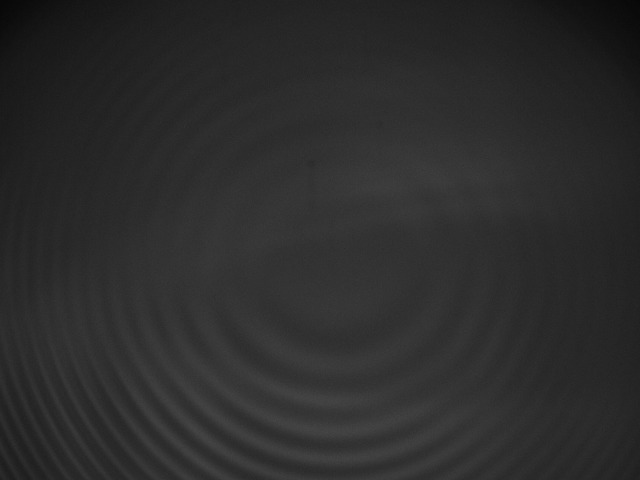
\includegraphics[scale = 0.1]{0.jpg}
    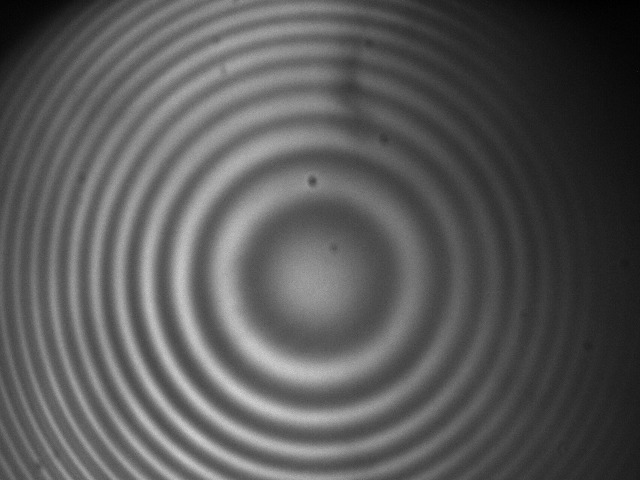
\includegraphics[scale = 0.1]{1.jpg}
    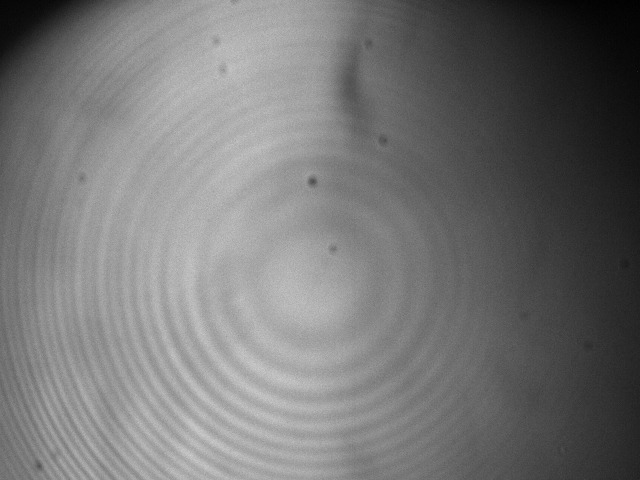
\includegraphics[scale = 0.1]{2.jpg}
    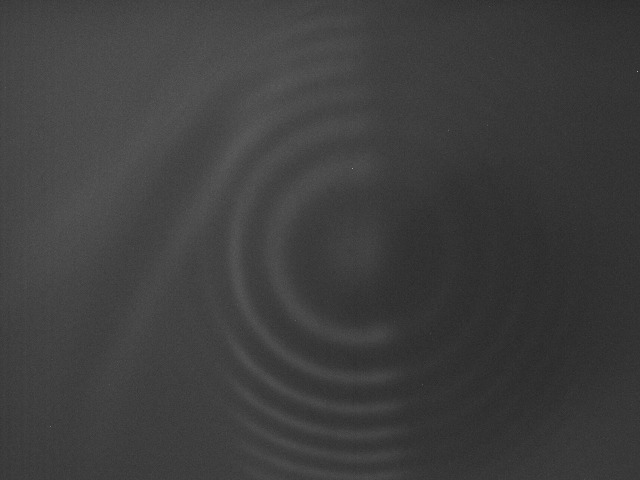
\includegraphics[scale = 0.1]{3.jpg}
    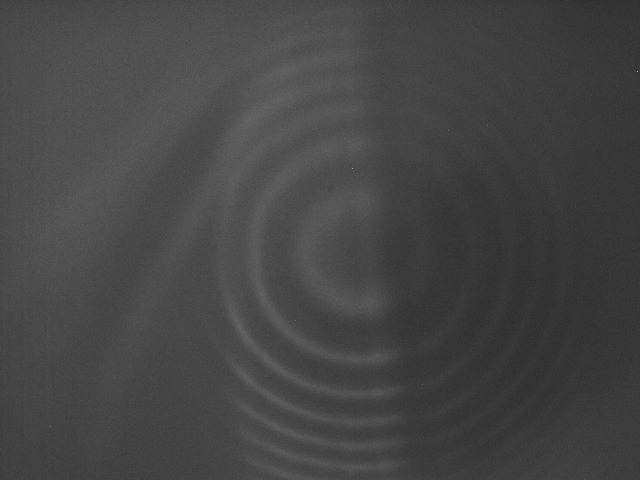
\includegraphics[scale = 0.1]{4.jpg}
    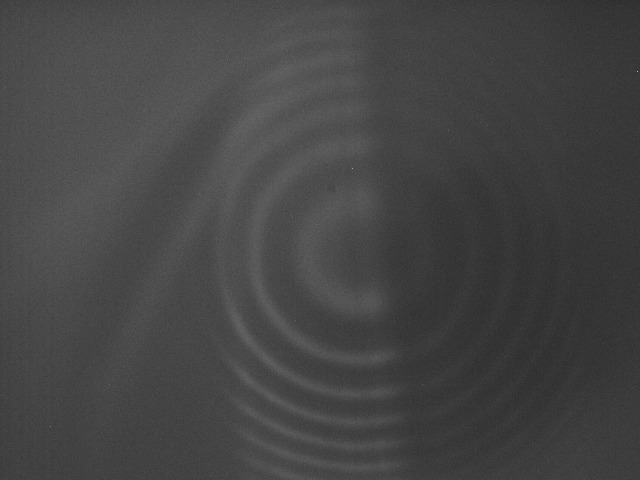
\includegraphics[scale = 0.1]{5.jpg}
    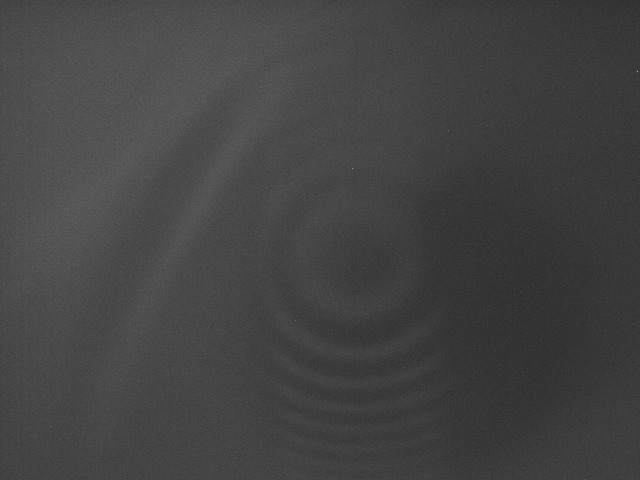
\includegraphics[scale = 0.1]{6.jpg}
    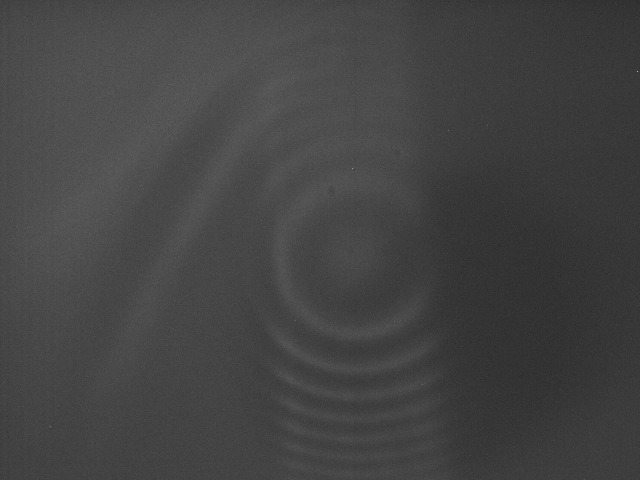
\includegraphics[scale = 0.1]{7.jpg}
    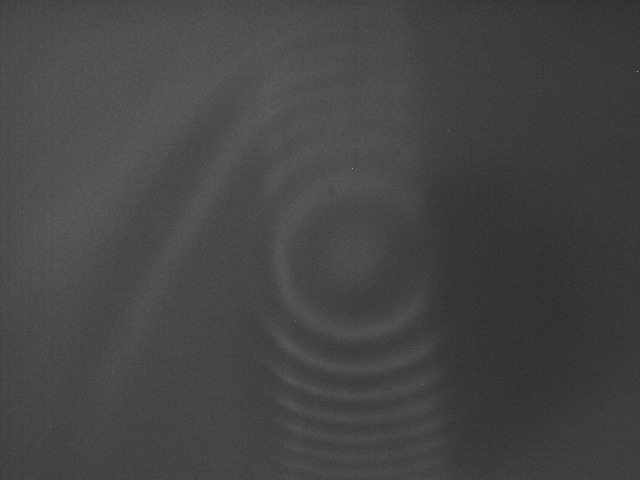
\includegraphics[scale = 0.1]{8.jpg}
    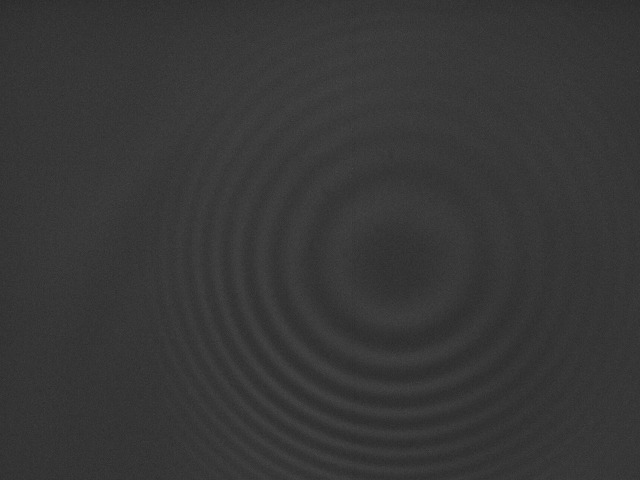
\includegraphics[scale = 0.1]{9.jpg}
    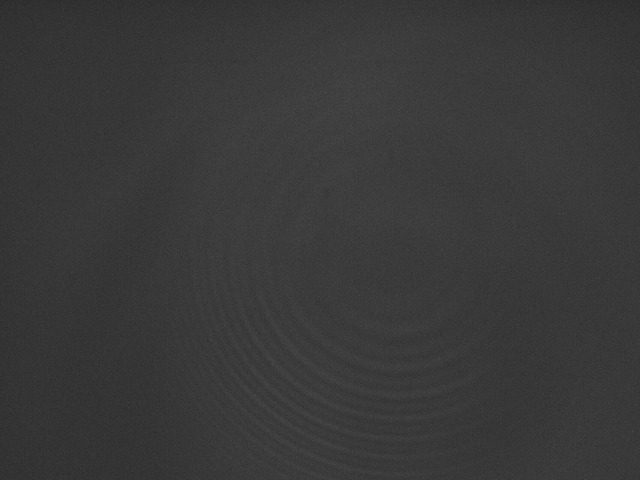
\includegraphics[scale = 0.1]{10.jpg}
    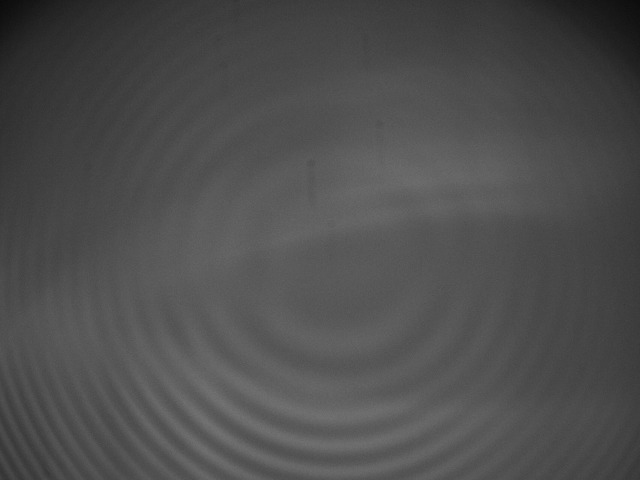
\includegraphics[scale = 0.1]{11.jpg}
    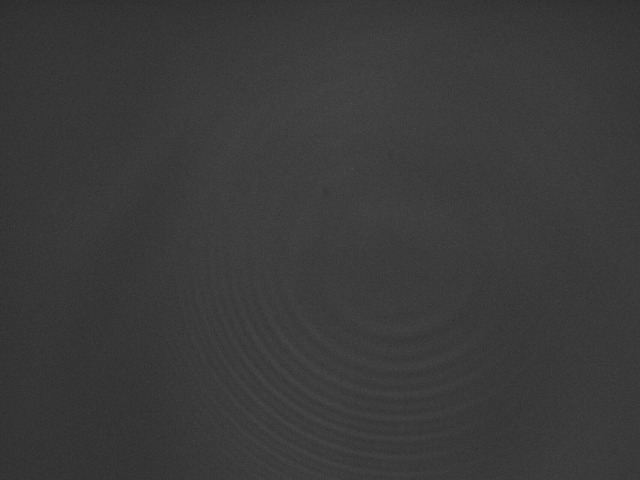
\includegraphics[scale = 0.1]{12.jpg}
    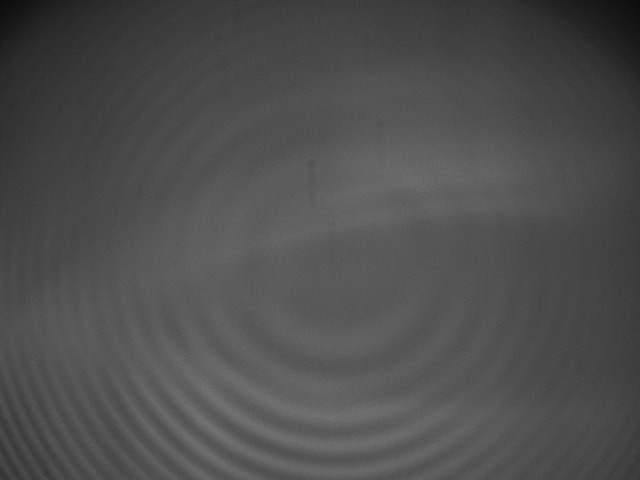
\includegraphics[scale = 0.1]{13.jpg}
    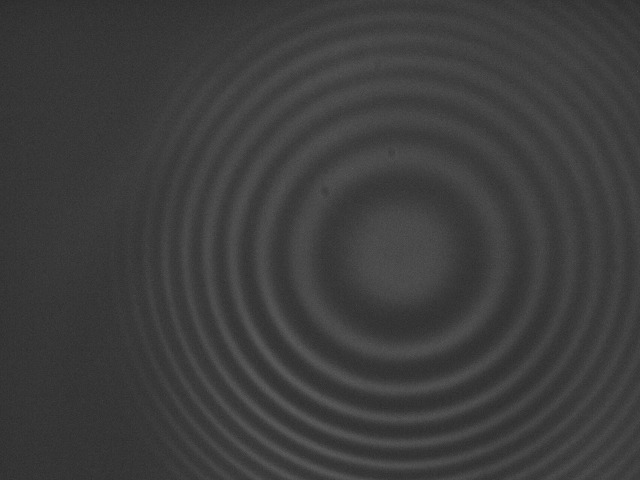
\includegraphics[scale = 0.1]{14.jpg}
    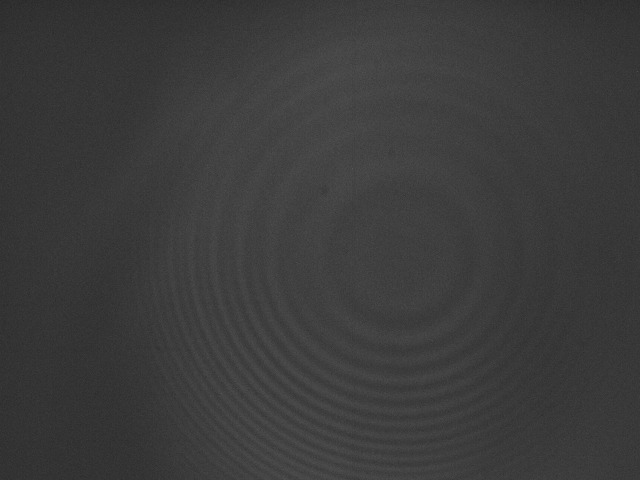
\includegraphics[scale = 0.1]{15.jpg}
    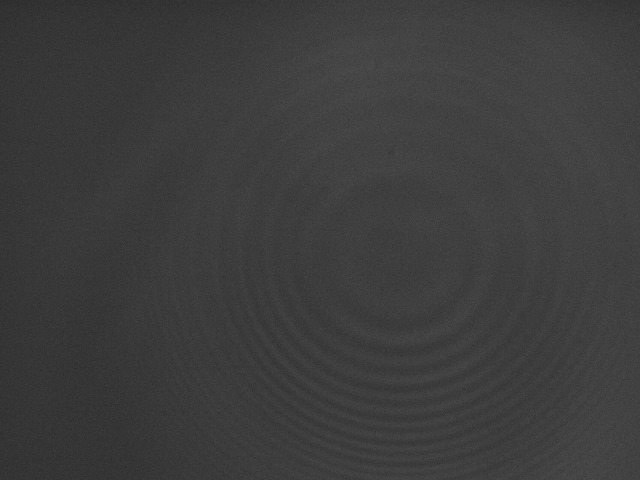
\includegraphics[scale = 0.1]{16.jpg}
    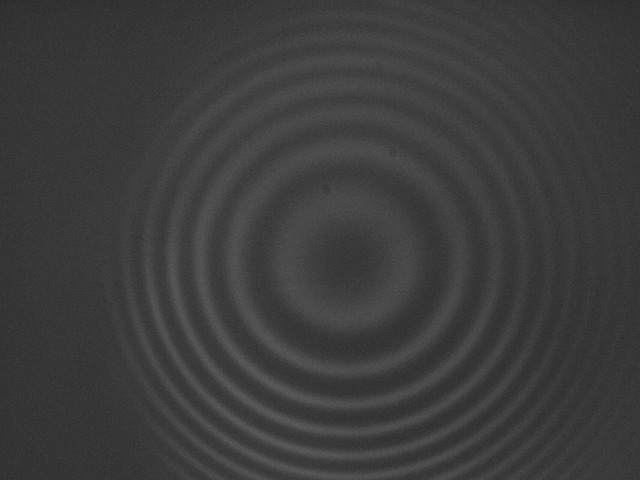
\includegraphics[scale = 0.1]{17.jpg}
    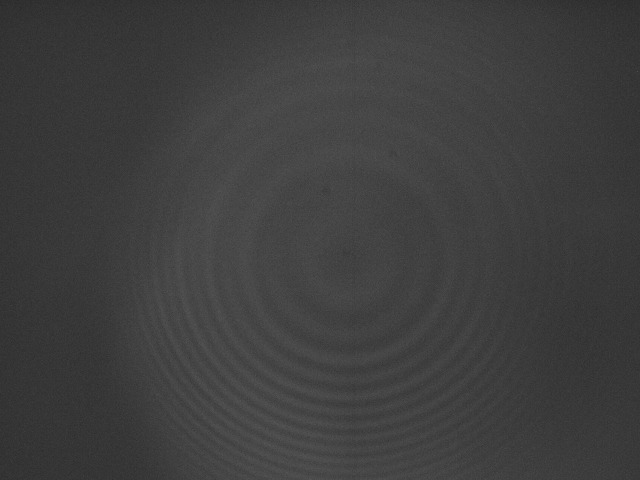
\includegraphics[scale = 0.1]{18.jpg}
    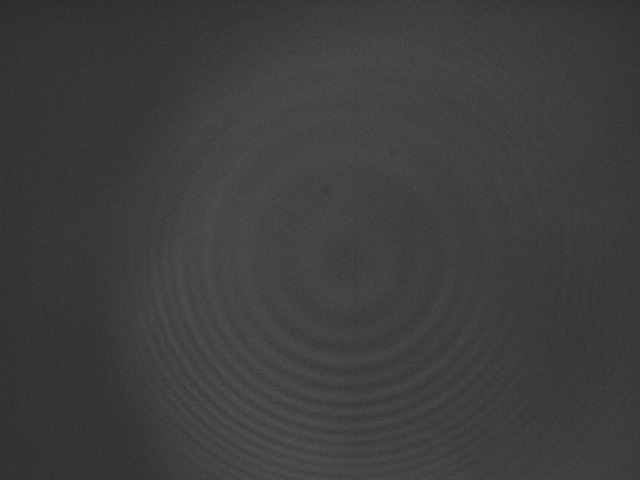
\includegraphics[scale = 0.1]{19.jpg}
    \caption{Raw Data for Balmer Series is in Calculations section}
    \label{fig:my_label}
\end{figure}




\end{document}
